%!TEX root = ../report.tex


% klar pointe: De væsentligste jobs i staten har tendens til at være lukkede om sig selv: det er i det private samt i de senere-statsliggjorte omsorgsjobs, der tidligere befandt sig i hjemmet, at der er cirkulation. 



%%%%%%%%%%%%%%%%%%%%%%%%%%%%%%%%%%%%%%%%%%%%%%
\chapter{Delanalyse 2: Forskellen på et delmarked og et segment er påvisningen af særegne (specifikke? partikulære) sociale processer indenfor delmarkedet \label{kapitel_delanalyse2_socialeprocesser}}
%%%%%%%%%%%%%%%%%%%%%%%%%%%%%%%%%%%%%%%%%%%%%%

Efter at have konstateret at der er en opdeling af arbejdsmarkedet for arbejdstagere i delmarkeder, hvor mobilitet indenfor delmarkederne er hyppig, og mellem delmarkederne sjælden, har dette kapitel til formål at besvare mit andet forskningsspørgsmål:

\begin{tcolorbox}[title=Forskningspørgsmål 2,
subtitle style={boxrule=0.4pt} ]
  Kan forskelle i de sociale processer vise, at der er tale om segmenter, og ikke blot delmarkeder?
\end{tcolorbox}

Dette forskningsspørgsmål vil jeg besvare ved at kigge på de sociale processer i delmarkederne, som jeg ser dem komme til udtryk gennem variablene indkomst, kønsfordeling, ledighedsgrad og faglige organisering, i den rækkefølge. For hver variabel præsenterer jeg nogle særlige kendetegn ved dens fordeling som helhed på arbejdsmarkedet, og derefter zoomer jeg ind på særlige delmarkeder for at understrege nogle pointer relateret til denne variabels fordeling på delmarkederne.  

Jeg afslutter delanalys1en ved at lave en sammenfatning af det billede, der tegner sig i kombinationen af de 4 variable, for at svare på forskningsspørgsmålet. 


%%%%%%%%%%%%%%%%%%%%%%%%%%%%%%%%%%%%%%%%%%%%%%
\section{Indkomstfordeling for alle \label{sec_delanalyse2_loen_alle}}
%%%%%%%%%%%%%%%%%%%%%%%%%%%%%%%%%%%%%%%%%%%%%%

j


\begin{figure}
\parbox[H]{8cm}{\null
  % \centering
  \captionof{figure}[Timelønninger farvelagt efter udvalgte percentiler]{Timeløn farvelagt efter udvalgte percentiler}
  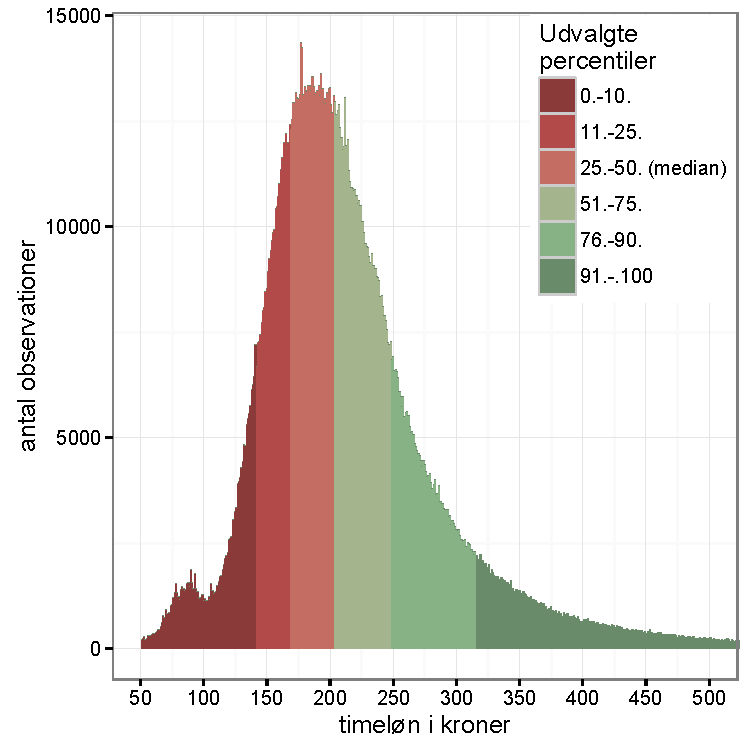
\includegraphics[width=7cm]{fig/deskriptive/timelon_quants_lowres2.pdf}
}
\parbox[H]{5cm}{\null
\centering
  % \vskip-\abovecaptionskip
  \captionof{table}[Centrale mål for fordelingen af timelønninger]{Centrale mål for fordelingen af timelønninger \label{delanalyse2_timelon_fordelingogfigur}}%
  \vskip\abovecaptionskip
%
% Table generated by Excel2LaTeX from sheet 'delanalyse2_indkomstfordeling'
\begin{tabular}{lr}
\toprule
Gennemsnit &                    222 kr.  \\
Sd-afvigelse &                      76 kr.  \\
\midrule
Mindste værdi &                      18 kr.  \\
Højeste værdi &                 2.155 kr.  \\
\midrule
10. percentil &                    155 kr.  \\
25. percentil &                    177 kr.  \\
Median &                    207 kr.  \\
75. percentil &                    243 kr.  \\
90. percentil &                    302 kr.  \\
\midrule
\textit{n} & \textit{205.798} \\
\bottomrule
\end{tabular}%

%
}
\end{figure}
%




Indkomstfordelingen i den arbejdende del af den danske befolkning kan ses i figur \ref{delanalyse2_timelon_fordelingogfigur} og tabel \ref{delanalyse2_timelon_fordelingogfigur}. 

\emph{\textbf{Til Jens: der skal skrives noget mere om her hvorfor at løn er vigtigt, fremfor bare at kaste sig ud i at lire tal af. - E}}



Vi kan se at fordelingen er nogenlunde centreret omkring gennemsnittet og medianen, hvilket også kommer til udtryk i standardafvigelsen på 76 kr/t. Stigningen i timeløn fra 100 kr/t til 175 kr/t er drastisk, mens faldet fra omtrent 200 kr/t og fremefter er noget mere støt i hældningen. Det kan man tolke sådan, at arbejdsmarkedsinstitutioner og overenskomster er ganske effektive til at regulere løndannelsen, således at lave timelønninger alligevel hindres i at ramme de niveauer, som fri prissætningen på arbejdskraften ville medføre. Det ses også, af den lange hale i timelønfordelingens øvre percentiler, at en lignende mekanisme ikke findes for de højere indkomster. Det danske skattesystems progressive beskatning af indkomst har selvfølgelig en hvis betydning, men det har ikke på samme måde en tydelig opdæmmende effekt, som vi ser, at der må findes for de lavere timelønninger. det er tydeligt, at timelønninger over den 90. percentil, tjener eksponentielt mere og mere frem mod den højeste timeløn på 4.492 kr.

Derudover findes der en lille pukkel af løninger på mellem 25 og 75 kr%
%
\footnote{ Grundet en teknisk fejl, der ikke blev rettet inden min forbindelse til registerdataen udløb, er lønninger mellem 25 og 50 kr/t ikke vist i grafen. Det betyder \emph{ikke} at de ikke er er tilstede i datamaterialet, blot at grafen ikke viser dem.}%
%
. Eftersom vores population er alle i arbejde melle 16 og 70 år, er der i de mange af disse tilfælde med stor sandsynlighed tale om ungdomsarbejde, samt enkelte fejlberegninger i . For en nærmere gennemgang af timeløns 

%%%%%%%%%%%%%%%%%%%%%%%%%%%%%%%%%%%%%%%%%%%%%%%%%%%%%%%%%%%%%%%%%%%%%%%%%%%%%
            \section{
%
            indkomstfordelinger på delmarkederne 
%            
            \label{sec delanalyse2 loen paa delmarkederne}}
%%%%%%%%%%%%%%%%%%%%%%%%%%%%%%%%%%%%%%%%%%%%%%%%%%%%%%%%%%%%%%%%%%%%%%%%%%%%%

Efter at have set på fordelingen af timelønninger generelt, skal vi nu se hvordan det er er differentiereret ud fra arbejdsmarkedets delmarkeder og klynger.  

I figur \ref{fig_analyse_deskriptivt_kort_timelon} er netværkskortet farvelagt således, at hvid markerer medianen på 208 kr/t. De røde farver er timelønninger under 208 kr/t. Jo mørkere rød, desto lavere timeløn. De grønne farver er over 208 kr/t. Jo mørkere grøn, desto højere timeløn%
%
\footnote{ Delmarkeder med en gennemsnitlig timeløn på 350 kr/t er sat til 350, da skalen ville blive spredt for langt ud for at imødegå disse outliers, hvilket ville gøre det svært at se nuancerne i forskellen mellem de timelønninger, som de fleste erhvervsgrupper trods alt har.}%
%
. Det ses at den grønne farves graduering er strukket længere end rød. Det er ikke overraskende, da vi netop ud fra figur \ref{delanalyse2_timelon_fordelingogfigur} kan se, at timelønninger strækker sig lagnt højere op over medianen end under den, bl.a. grundet det danske arbejdsmarkedes indretning, som argumenteret for i beskrivelsen af figur \ref{delanalyse2_timelon_fordelingogfigur}.

%
\newgeometry{left=-0.01cm,bottom=0.1cm}
\begin{figure}[H]
\begin{center}
  \caption{Intern mobilitet for klyngerne.}
  \label{fig_analyse_deskriptivt_kort_timelon}
  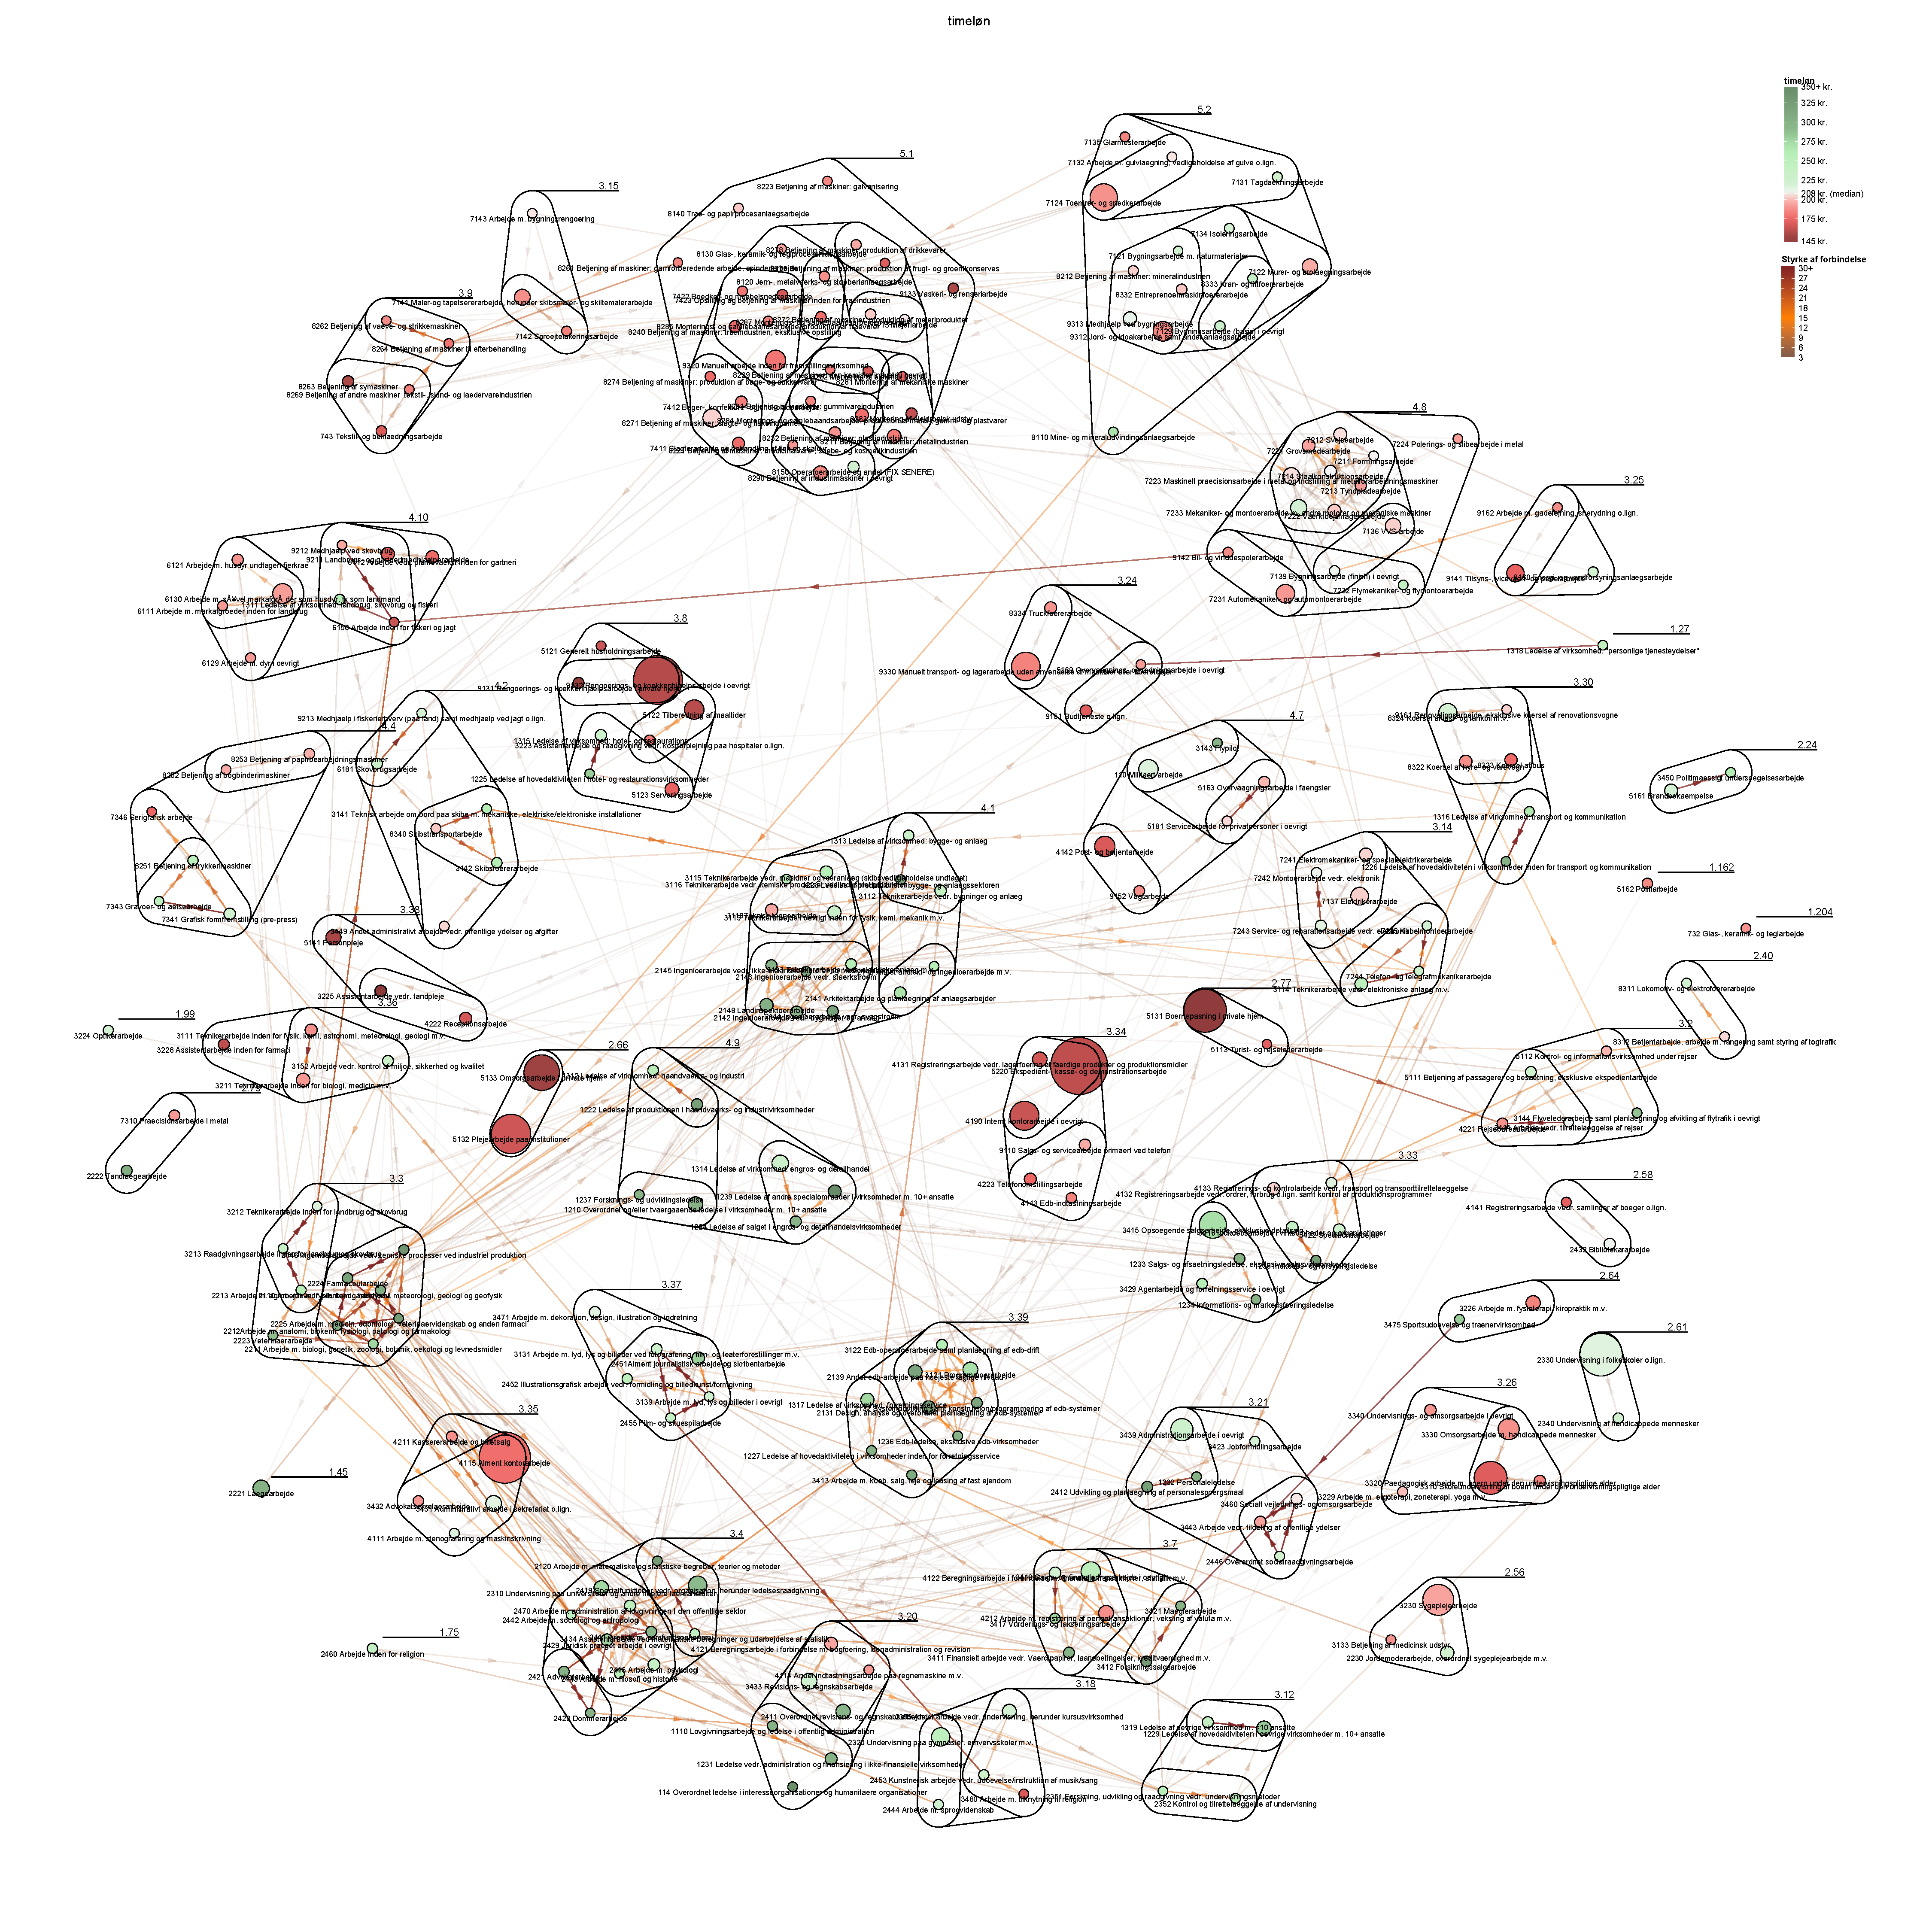
\includegraphics[width=1.0\textwidth]{fig/netvaerkskort/kort_timelon.pdf}
\end{center}
\end{figure}
\restoregeometry
%

Det overordnede netværkskort præsenteret her, giver os allerede en ide om en vis systematik i lønforholdene i forskellige placeringer på arbejdsmarkedet. Det er velkendt at kortets delmarkeder er lavet ud fra mobilitet mellem erhvervsgrupperne. Selve placeringen \emph{af} delmarkederne på kortet er imidlertidig også sket ud hvilken mobilitet der findes \emph{mellem} klyngerne. Derfor er det interessant, at vi ser en rødlig halvmåne forme sig i venstre side af kortet, mens en - lidt mindre - grøn formation findes i højre side. Ved at se på forbindelserne kan vi straks konstatere hvorfor, at kortet ser ud som det gør: Mellem de grønne, velbetalte delmarkeder ser vi meget kraftige forbindelser mellem delmarkederne. 

De 18 delmarkeder, der her er tale om, befinder sig stort set alle i Disco-hovedgruppe 1, 2 eller 3. Hvilket vil sige erhverv med høje (boglige) uddannelseskrav, og/eller meget ledelsesansvar. 

Der kan være to årsager til hvad vi ser på kortet: 1) Enten er udvekslingen af arbejdskraft på tværs af delmarkeder langt mere hyppig, eller 2) udvekslingen er mere specifik: Forbindelserne på kortet viser de kraftigste forbindelser, ikke alle forbindelser, og derfor vil mobilitet, der er mere jævnt fordelt, forblive usynlig på (denne udgave af) kortet. Ved at se på den interne mobilitet for sig for henholdsvis de 18 delmarkeder i den grønne formation for sig, og den røde halvmånes 36 delmarkeder for sig er det muligt at svare på. Den grønne formation har en gennemsnitlig intern mobilitet på 80 \%, og den røde halvmånes er på 77 \%%
%
  \footnote{ Det samme gælder for medianen og standardafvigelsen: Den røde halvmåne har en noget højere standardafvigelse og lavere median, men kun et par procentpoints forskel.}%
%
. Der er altså ikke tale om en væsentlig forskel i intern mobilitet mellem de to formationer. De kraftigere forbindelser i den grønne formation skyldes derfor, at den mobilitet, der findes, foregår langt mere struktureret langs bestemte linjer på tværs af delmarkederne. Den røde halvmånes mobilitet er “smurt tyndere ud”, og derfor ses den ikke på kortet%
%
 \footnote{ I appendiks \ref{app_netvaerkskort}, figur \ref{appendiks kort edges} findes et kort der viser alle forbindelserne, hvor dette kan ses.}%
%
.Sikft mellem den grønne formation af delmarkeder, med lange boglige uddannelse og/eller meget ledelsesansvar i højere grad sker via bestemte kanaler end tilfældet er i de resterende delmarkeder. Det er interessant, da det der netop karakteriserer den grønne formation, er at deres lønniveauer befinder sig i den bedst betalte halvdel af befolkningen. 

Hvis man skal komme med en tentativ analyse af hvad denne forskel i mobilitetsstruktur \emph{kan} betyde for den politiske orientering, erindrer læseren muligvis Claus Hjort Frederiksens udmelding som beskæftigelsesminister i 00'erne (find præcis årstal senere \#todo), hvor han kom i vælten ved at udtale, at hvis man med en lang videregående uddannelse ikke kunne finde job, skulle man finde arbejde i netto eller blive postbud i stedet. Det udløste et ramaskrig. Blandt dem med lang videregående uddannelse. Mens det for ikke-boglige klasser sandsynligvis var en ganske tilfredsstillende udmelding, og det er nok ikke usandsynligt, at udtalelser som denne, der gjorde Venstre til et bredt funderet parti i 00'ernes Danmark. Mit kort giver en troværdig forklaring på hvorfor, Da det ses, at netop erhvervsgrupper med lange videregående uddannelser, er vant til at søge beskæftigelse indenfor andre delmarkeder i langt mere strukturede baner end resten af delmarkederne. Det er denne form for kulturkrig, sociologen Thomas Frank beskriver i sin bourdieu-inspirerede klasseanalyse i bogen “What's the Matter with Kansas? - how the conservatives won the heart of America” fra \citeyear{Frank2007}. i Norge udkom en lignende bog i \citeyear{Marsdal2007} med en identisk Bourdieau-analyse, skrevet af journalisten Magnus  Marsdahl. Analysen er kort sagt, at venstrefløjspartierne er blevet til de boglige klassers parti. Det lukrerer de borgerlige politikere på ved at markerer sig med forslag og udtalelser, der er på kant med de “dannede” sociale gruppers verdensbillede, hvilket de naturligvis reagerer på med deres lærde sprog. Disse udmeldinger viser venstrefløjens traditionelle arbejderklasse, at den verden, hvori de venstreorienterede værdier står stærkt, ikke er deres verden. 

Det er selvfølgelig et noget stort brød at slå op, og jeg påstår ikke at den her fundne struktur kan bære en sådan bevisbyrde alene. Jeg vælger alligevel at præsentere den her, da jeg dog mener, at det netop er sådanne oplevelser af arbejdet, der giver et blik på verden, der kan formes til forskellige politiske perspektiver. Det er min overbevisning, at politiske værdiorienteringer ikke har samme kobling til arbejdslivet som tidligere, hvilket er et velfunderet empirisk standpunkt indenfor sociologisk og politologisk forskning (henvisning til Scott \#todo). Det betyder imidlertidig ikke, at politisk værdiorientering er \emph{af}koblet fra arbejdslivet, men at en række komplekse ændringer af parti, klasse og forbrugskulturen gør disse sammenhænge anderledes end tidligere. Som valget af Trump i november 2016 viste, er klasse stadig en relevant faktor, hvis man forstår hvad det betyder i dag (link til artikel fra Trumps datahold og så noget mere substantielt der viser at analytikerne tog fejl). Den her fremførte tolkning er et eksempel på hvorledes en oplevelse af arbejdslivet kan understøtte moderne sociologisk fundererede analyse om politisk værdidannelse ud fra moderne klasseteori, såsom Thomas Franks og Magnus Marsdahls analyser.



 % find ud af hvor meget mobilitet der "mellem" de to delmarkeder. \#todo 

%
\subsection{To delmarkeder i hver sin ende af indtjeningsspektret}
%

Hvilke delmarkeder har en høj timeløn og hvilke delmarkeder har en lav timeløn? Med andre ord - hvis vi starter helt naivt - er der bestemte typer arbejde, der er lønnes højt og lavt? Hvis vi antager, som Goldthorpe og Oesch gør det, at forskelligt arbejde indeholder forskellige sociale processer, må det være muligt at se dette afspejlet i delmarkedernes arbejdsindhold, samt hvor ens eller forskellige lønningerne er indenfor delmarkederne. 

 For at illustrerer det vil jeg zoomer ind på to delmarkeder, hvoraf et befinder sig i lave ende af timelønningerne og den anden i den højeste ende.

%
\subsubsection{Delmarked 3.35}
%



 Det første jeg vil fremhæve er delmarked \emak{s3.35}. Dette delmarked indeholder lavere grads servicejobs, og er det lavest lønnede delmarked, der består af > 2 erhvervsgrupper. Den gennemsnitlige timeløn, som aflæst i tabel, er på 175 kr/t, med en standardafvigelse på kun 14 kr/t. Der er tale altså tale om et delmarked, hvor gennemsnitslønnen er lav, og den er stabilt lav for alle de erhvervsgrupper, det består af. 
 % skal jeg lave en tabel med discogrupperne eller kun for segmentet? find ud af det senere \#todo

% Erhvervsgruppen består af jobbene telefonsælger, interviewer, pølsemand, klunser samt skopudser
Arbejdet i delmarkedet består af servicerelatereret arbejde, administrativt arbejde og kundepleje(?), og har ikke høje uddannelseskrav. Overraskende nok er det \emak{d9110} der har den højeste lønning på 197 kr/t. Det er overraskende, fordi erhvervsgruppen slet ikke har nogle uddannelseskrav, og er derfor i DSTs opdeling “færdighedsløst” arbejde. Denne erhvervsgruppe har dog også en intern højstandardafvigelse på 78 kr/t, den højeste i delmarkedet. Det giver god mening, da man må formode at der er stor forskel på at sælge hårde hvidevarer og sælge tekniske produkter til et nichemarked, hvor der kræves en vis teknisk kompetence for at kunne udtale sig om dets specifikationer. 

%
\begin{wrapfigure}{l}{6cm}
  \vspace{-20pt}
  \begin{center}
    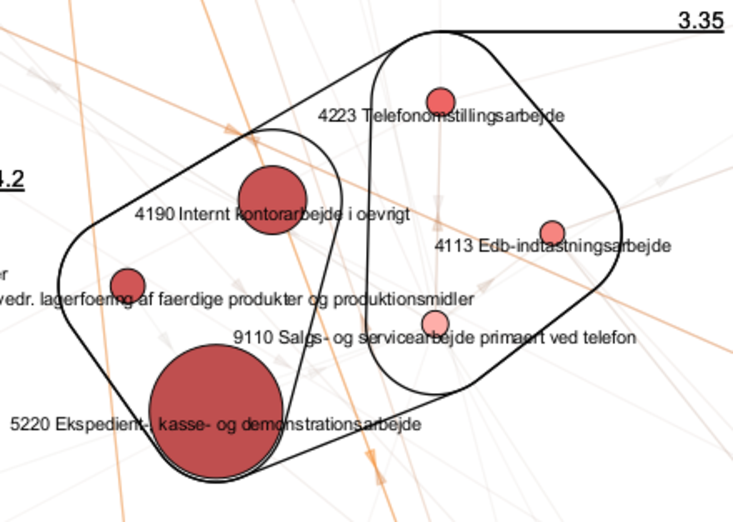
\includegraphics[width=6cm]{fig/segzoom/seg_3_35_timeloen.pdf}
   \caption{}
   \label{fig_delanalyse1_zoom_3_35}
  \end{center}
  \vspace{-20pt}
\end{wrapfigure}
%

Delmarkedet er interessant af to simple årsager ud kvantitative mål, samt en enkelt teoretisk, der vokser ud af disse to. 

For det første indeholder den største enkeltstående erhvervsgruppe, \emak{5220},  der indeholder 5 \% af alle beskæftigede på det danske arbejdsmarked. Der er tale om en samling af jobs, der indeholder en lang en lang række ekspedientarbejde, såsom blomsterekspedient, købmandsekspedient, bilsælger og togsteward. Altså arbejde, hvor man sælger til, eller ekspedierer, kunder ansigt-til-ansigt. 

For det andet, grundet denne erhvervsgruppe er \emak{s3.35} det største delmarked, med 8 \% af det totale antal beskæftigede. Det er samtidig det delmarked, der har den ubetinget højeste andel af den totale mobilitet, på 8,8 \%, hvilket er 2,8 \% mere end det næststørste delmarked. 

For det tredje understøtte det Oesch tese om at skiftet fra produktion af fysiske varer til servicerelateret arbejde har betydning for klassestrukturen. Det er for tidligt at gå ind i endnu, men det er interessant, at det største \emph{og} lavest betalte delmarked er servicerelateret arbejde, hvis genstandsfelt er salg af varer til almindelige forbrugere. 

De nederste manuelle arbejdere i delmarked \emak{s5.1} der primært arbejder med betjening af maskiner i industriproduktionen, har faktisk en timeløn, der ligger 10 kr højere. Jeg vil uddybe dette senere, efter jeg har taget fat på hvad Oesch peger på som det andet vigtige parameter for den ændrede klassestruktur, som er kvindernes indtog på arbejdsmarkedet fra midten af det 20. århundrede og frem. 





%interessant nok er de også delt op i flere kategorier på 4-cifret niveau, hvor butiksassistent, blomsterekspedient, bilsælger etc er i samme kategori. Måske en blind vinkel i ISCED-klassifikationen. 
% dog ligger timelønnen for individer i segmentet på 264 i 3.35 og nærmest det samme i 5.1. jeg bruger gennemsnittet af erhvervsgrupper i stedet for individer fordi erhvervsgrupper er min analyseenhed, fuck individerne. det har den praktiske konsekvens at antallet af individer indenfor erhvervsgrupperne ikke medregnes i gennemsnittet for klyngerne, dvs hvis en af de erhvervsgruppe, dvs en af de 8 erhvervsgrupper, der indeholder < 600 personer var placeret i samme segment som en af de 8 erhvervsgrupper, der indeholder < 50.000, så ville gns for f.eks. løn være det samme.




%
\subsubsection{Delmarked 4.9}
%

Med 333 kr/t er delmarked \emak{s4.9} det bedst indtjenende delmarked i byen. Det indeholder $\nicefrac{1}{4}$ af erhvervsgrupperne i Discos hovedgruppe 1, som består af ledelse på øverste plan. Det har samtidig den 2. højeste standardafvigelse på 85 kr/t, så indtjeningen erhvervsgrupperne i mellem er meget varieret.  

% skriv noget her om ledelsesarbejde. Læs om ledelsesarbejde!           

Det er ikke overraskende at “ledelsesdelmarkedet” indtager denne position i indtjening. Det interessante er snarere, at de  resterende $\nicefrac{3}{4}$ indenfor ledelse på højeste plan er tilknyttet de delmarkeder, der relaterer sig til ledelsens genstandsfelt. Med andre ord er \emak{d1236} tilknyttet delmarked \emak{s2.31}, der har at gøre med det IT-udviklingsarbejde, der befinder sig på det “højeste” faglige niveau. Interessant nok gælder det også Disco 1-erhvervsgrupper, hvor det er ledelse af produktion, hvis arbejdskraft kræver mindre eksklusive kompetencer end i delmarkedet beskæftiget med IT-udvikling på højeste niveau. Eksempelvis landbrug, restauration og  %det skal nok ikke stå her, faktisk. 

%Måske skal jeg skrive om et andet delmarked i stedet, et der giver bedre mening. Hmmm. 


%
\begin{wrapfigure}{r}{6cm}
  \vspace{-20pt}
  \begin{center}
    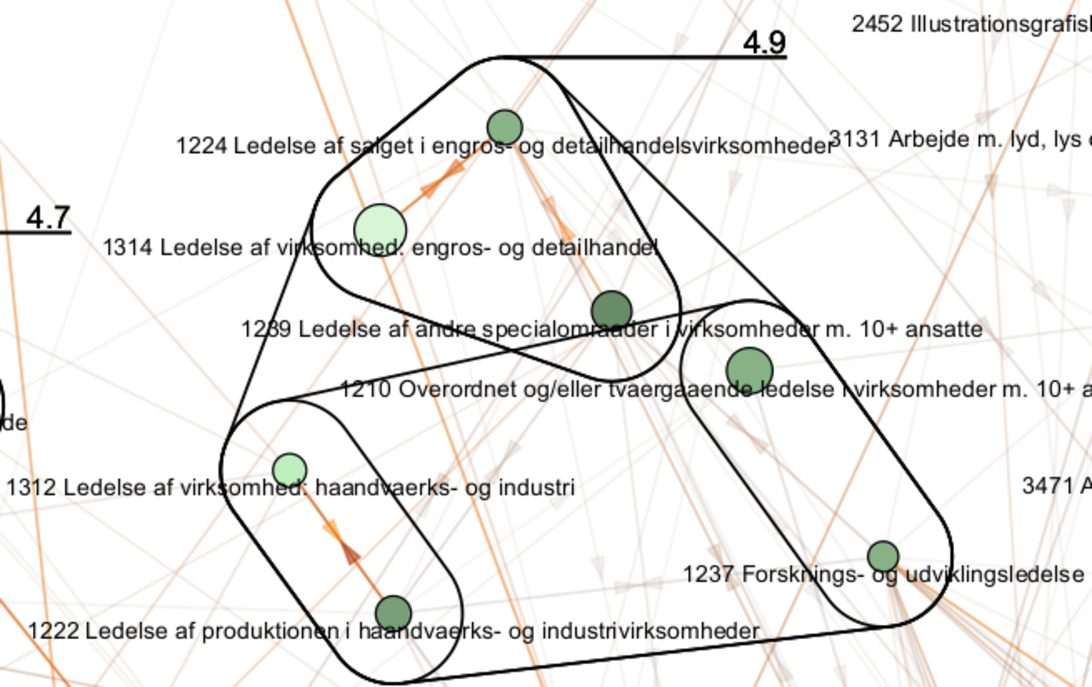
\includegraphics[width=6cm]{fig/segzoom/seg_4_9_timeloen.pdf}
   \caption{}
   \label{fig_delanalyse1_zoom_4_9}
  \end{center}
  \vspace{-20pt}
\end{wrapfigure}
%



\pagebreak 
%%%%%%%%%%%%%%%%%%%%%%%%%%%%%%%%%%%%%%%%%%%%%%
\section{Det kønsopdelte arbejdsmarked \label{sec_delanalyse2 koensfordeling generelt}}
%%%%%%%%%%%%%%%%%%%%%%%%%%%%%%%%%%%%%%%%%%%%%%

% først graf der viser stigning gennem min periode. citat om at kvindelig employment har været den største faktor employment i 80'erne og de tidlige 90'ere i vesteuropa, citat s. 33 Oesch.



Netværkskortet i figur \ref{fig_delanalyse1_kort_koen} på s. \pageref{fig_delanalyse1_kort_koen} viser kønsfordelingen på arbejdsmarkedet. Selv ved første øjekast, er det tydeligt at køn er en klar differientieringsfaktor. 
En vigtig pointe, der kan ses ud fra kortet, men let kan overses: Det er også tydeligt, at placeringen af delmarkederne på kortet heller ikke lader til at være tilfældig i forhold til kønssammensætningen. 

De fleste delmarkeder med en markant overrepræsentation af kvinder befinder sig i toppen af kortet. Disse delmarkeder er alle beskæftigelser i servicesektoren. Enten indenfor administrativt arbejde, omsorgsarbejde, pædagogik, kundepleje eller arbejde, der traditionelt har været kvindeligt husarbejde, såsom rengøring og tilberedning af måltider.  

Til højre for kortets midte, er der en række delmarkeder med et miks af erhvervsgrupper med enten svag overrepræsentation af mænd eller af kvinder. De nederste - \emak{s4.11} og \emak{s3.4} - har flest erhvervsgrupper med mænd, mens de øverste - eksempelvis \emak{s3.21} og \emak{s3.18} - har flest erhversvgrupper med kvinder. 

Nederst i kortet har vi det tradtionelle mandearbejde. Kortet viser tydeligt, at hvis vi med “traditionelt” mener “statistisk”, er arbejde af denne karakter stadig mandearbejde. Der er tale om fag indenfor manuelt arbejde, som er praktisk/produktionsmæssigt orienteret. Overordnede labels, man kan sætte på denne type arbejde er: landbrugsproduktion, transport af varer, bygge-anlægsarbejde, reparation/vedligehold af maskiner eller industriapparater, samt den brede vifte af teknikerarbejde, hvis genstandsfelt kan være gas, kemi, svag- og stærkstrøm. Samt ikke mindst: Ledelsesarbejde. Ingen af de 27 erhvervsgrupper indenfor Discos hovedgruppe 1 har en andel af kvinder på over 50 \%. Af disse 27 erhvervsgrupper har 59 \% en andel af kvinder på under 25 \%. Dette aflæses let i kortet, hvor selv delmarkeder, der har en overvægt af kvinder i alle dets erhvervsgrupper, stadig har mænd i ledelsespositionerne indenfor delmarkedets funktionsområde.  % de dækker 5 % af de beskæftigede. pointe der skal med? Måske et andet sted i stedet?  % husk at definer funktionsområde. Måde at tale om arbejde på, kulturfunktionalistisk, a la Grusky. \#todo


%
\newgeometry{left=-0.01cm,bottom=0.1cm}
\begin{figure}[H]
\begin{center}
  \caption{Kønsfordeling på arbejdsmarkedet}
  \label{fig_delanalyse1_kort_koen}
  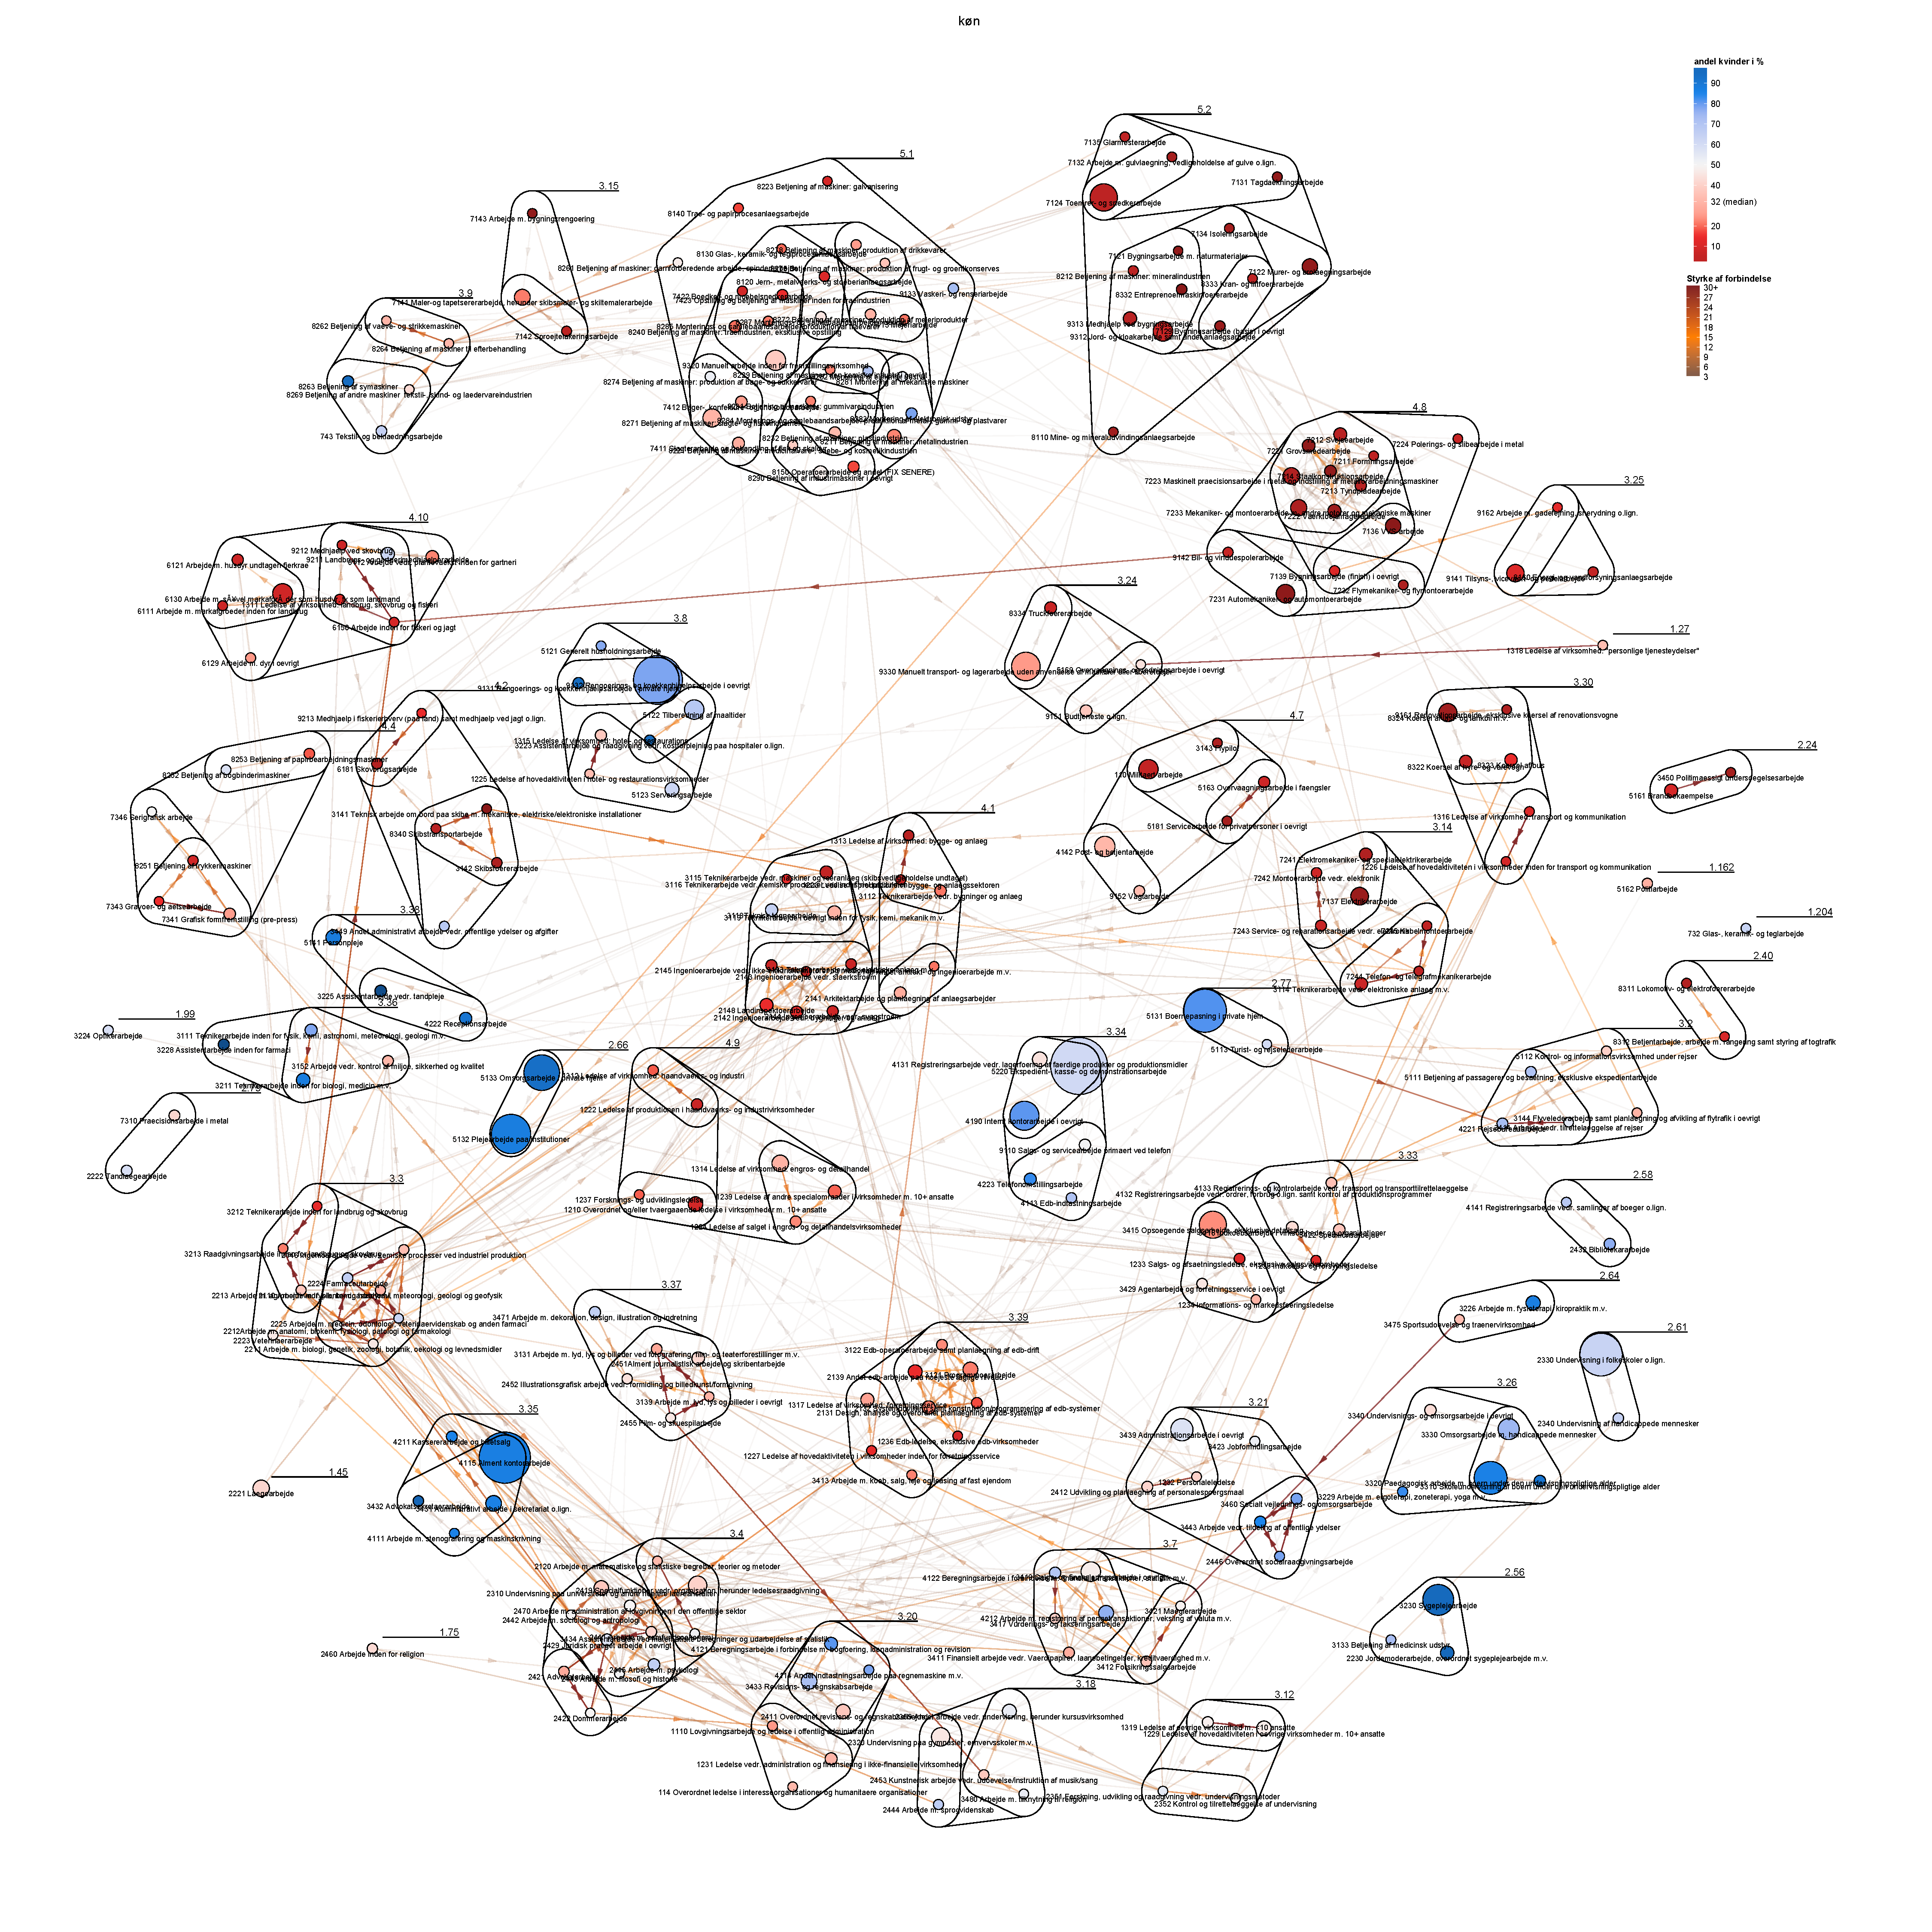
\includegraphics[width=1.0\textwidth]{fig/netvaerkskort/kort_koen.pdf}
\end{center}
\end{figure}
\restoregeometry
%



% udbudssiden er højere uddannelsesniveauer for kvinder, og steps toward equal right. på efterspørgselssiden er det væksten i servicejobsne der står for det. integrationen af husholdningsaktiviter i markedet og statsforbrug i offentlig sundhed og uddannelse har ændret efterspørgslen efter arbejdskraft og særligt kvindelig arbejdskraft markant. s. 33-4 

% På demand siden


% for klasseteori styrker casen for at den rette observationshed for klasse er individet, og ikke husholdningen. Mænds distribution på arbejdsmarkedet er anderledes end kvinders, og skal derfor forstås ud fra forskellige oplevelser af arbejdslivet. Når så mange kvinder arbejder i servicefag, er en opdeling baseret på manufaktur ikke til meget nytte når de skal placeres i et klasseskema. s. 35

% Dette betyder også et skift fra hierarkisk stratifikation til horisontal stratifikation. 

% fokus på husstand som observationsenhed eller individet stor splittelse i 80'erne. Mener med en vis form for konsensus om hvad formålet er, om det er at se på markedssituationen eller på arbejdssituationen. Individet er at foretrække på arbejdssistuationen, og det er den, jeg også vil fokusere på her. s. 42. 

% "there are no grounds for regarding the lower leve ls o f  then on-manuel  hierarchyas somehow superior to manuel work" s. 46

% Introduktionen af nye teknologier og automatiseringer gør at skellet mellem white-collar og blue-collar ændrer sig, den sociale distance mellem de to bliver anderledes. 


%
\subsection{udvalgte delmarked: Klynge 3.4}
%

Delmarked \emak{s3.36} er den del af det danske arbejdsmarked, der varetager repetetivt adminstrativt arbejde, af generisk karakter, eksempelvis jobbet sekretær. Det er arbejde, der er påkrævet i langt de fleste moderne virksomheder, organisationer og statslige instutitioner. Med en andel af kvinder på 88 \% har \emak{s3.36} den  3. højeste andel af kvinder blandt alle delmarkeder, og indeholder 5,7 \% af alle beskæftigede. 

Delmarked \emak{s5.2} er det omvendte forhold, og indeholder med sin andel på 2,5 \% kvindelige lønmodtagere den 2. laveste andel på arbejdsmarkedet. Dette delmarked kan ud fra erhvervsgrupperne i det, hurtigt karakteriseres som delmarbejdet for bygge-anlægsarbejde. % og indeholder 4,7 \% af alle beskæfigede. 

\begin{figure}
\parbox[H]{7cm}{\null
  \centering
  \captionof{figure}{Delmarkedet for alment kontorarbejde (\emak{s3.36})}
  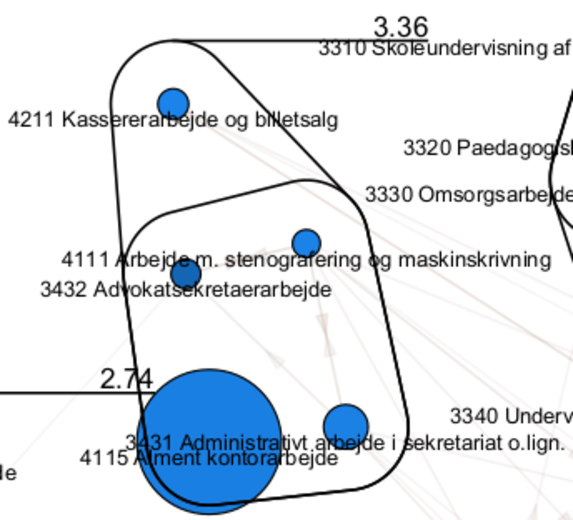
\includegraphics[width=6cm]{fig/segzoom/seg_3_36_koen.pdf}
}
\parbox[H]{7cm}{\null
\centering
  % \vskip-\abovecaptionskip
  \captionof{figure}[t]{Bygge-anlægsdelmarkedet (\emak{s5.2})}%
  \vskip\abovecaptionskip
%
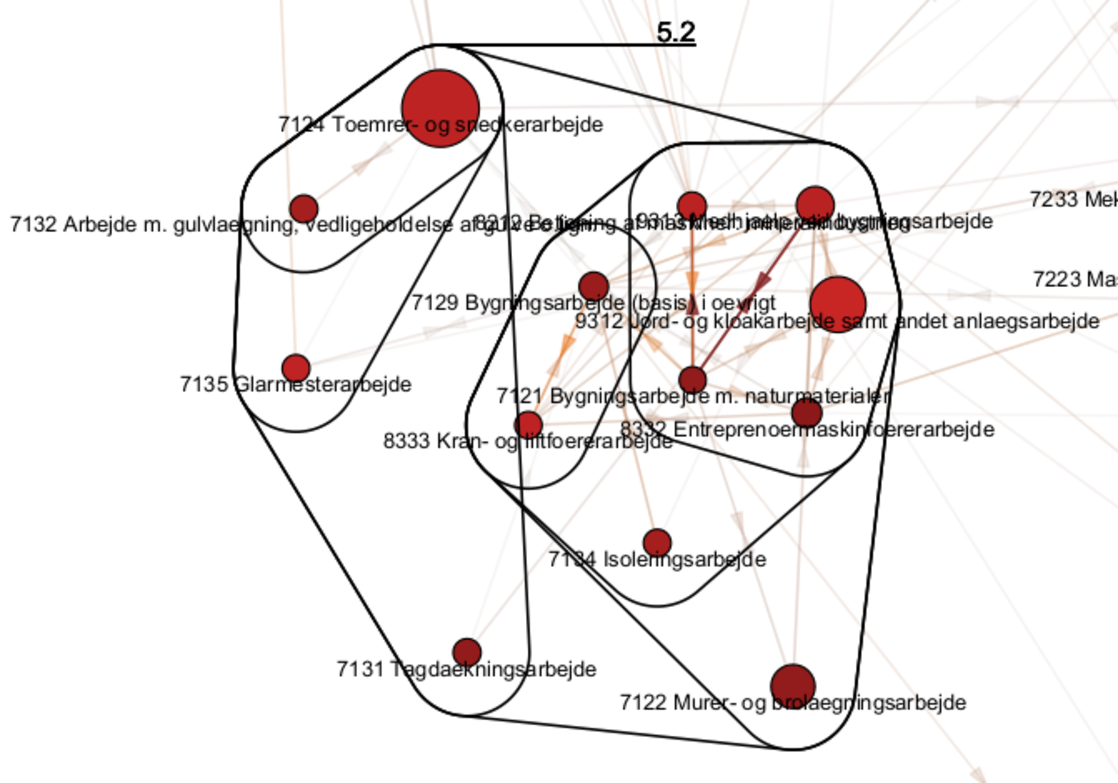
\includegraphics[width=8cm]{fig/segzoom/seg_5_2_koen.pdf}
%
}
\end{figure}
%

Det sidste delmarked jeg vil fokusere på udelukkende i et kønsperspektiv er delmarked \emak{s3.4}. Her er kønsfordelingen næsten 50/50, dog med en svag overvægt af mænd. 

Alle erhvervsgrupper i delmarkedet undtagen \emak{d3434} kræver færdigheder på højeste niveau indenfor ISCED kategoriseringen. Det er arbejde, der har en høj grad af specialisering, og kræver længere videregående uddannelser. De samfundsmæssige funktioner i dette delmarked kan deles op i følgende fire typer:

%
\begin{wrapfigure}{r}{6cm}
  \vspace{-20pt}
  \begin{center}
    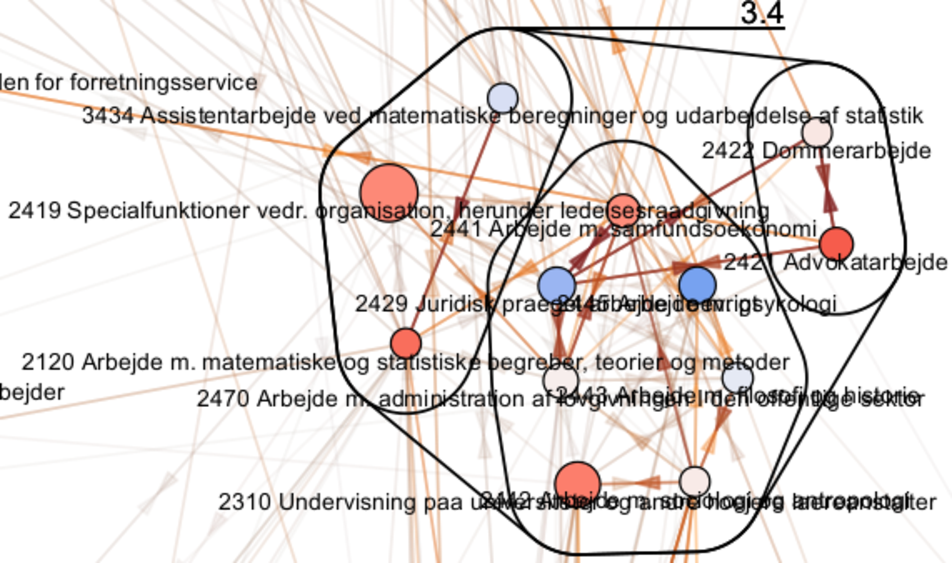
\includegraphics[width=6cm]{fig/segzoom/seg_3_4_koen.pdf}
   \caption{}
   \label{fig_delanalyse2_zoom_3_4 koen}
  \end{center}
  \vspace{-20pt}
\end{wrapfigure}
%



%
\begin{itemize}
 \itemsep -0.5em
   \item Varetagelse af og beskæftigelse med statens love.
   \item Beskæftigelse med samfundsøkonomien, både i form af nationaløkonomiske hensyn, men også i form af kompetencer indenfor finans- og erhvervsøkonomi og andre konsulent-stillinger%
   %
   \footnote{ \label{d2419 forklaring} På det 6-cifrede Disco-niveau indeholder \emak{d2419} både jobs såsom byggesagkyndig og regionschef, altså primært statslige regulative funktioner. Men \emph{også} finanseringskonsulent, erhvervskonsulent samt markedsanalytiker. Man skulle umiddelbart tro at disse funktioner ville tilhøre “finanseringsdelmarkedet” \emak{s3.7}, men det er ikke tilfældet. Sandsynligvis på grund af de tidligere nævnte jobs. Man kan være skeptisk overfor om DST har lavet en fornuftig aggregering på det 4-cifrede niveau i dette tilfælde.}%
   %
   \item Forskning og viden om “ indflydelsen på mennesket selv, ved dets stofskifte med verden”%
   %
   \footnote{ som Marx kunne have formuleret det.}%
   %
    : Historikere, sociologer, filosoffer, antropologer og psykologer.    
   \item Uddannelse af den næste generation af samfundets højest uddannede erhvervsgrupper. 
\end{itemize}
%

Det er tydeligvis arbejde, der må antages at have en vis status tilknyttet, hvilket også kan ses i lønniveauet - mere om det i (reference her til label for det kapitel \#todo).  Det ser ud til, at arbejde med blandet kønsfordeling har tendens til foregå blandt de højere uddannelser, og særligt indenfor felter, der - i en Bourdieu-optik - kan siges at have (blah blah find Bourdieu i DDS Stine Faber-teksten \#todo). Men det ses at dette sker indenfor specifikke arbejdsområder, og ikke andre. Det er ikke alle højere uddannelser, at vi ser denne jævne kønsfordeling, der sjovt nok er karakteriseret ved ikke at være såkaldte \emph{hårde} videnskaber%
%
\footnote{ Sprogligt er det selvfølgelig interessant at de netop kaldes de \emph{hårde} videnskaber. Jeg mener ikke det er urimeligt at se på dette som et udtryk for den kønnede arbejdsdeling: Mænd arbejder med \emph{hård} videnskab, og de laver \emph{hårdt} fysisk arbejde, og så videre.}%
%
 . 



Som ovenstående gennemgang har vist, er den kønsmæssige arbejdsdeling tæt bundet op på delmarkedernes grænser. De steder, hvor kønssammensætningen er jævn, er bestemte områder af den samfundsmæssige arbejdsdeling, og kan ikke siges at være udtryk for tilfældigheder, da der findes gode fortolkninger til at forklare hvorfor vi ser den lige kønssammensætning i netop disse delmarkeder. Det samme gælder også de kønsopdelte delmarkeder.

I det forskningsspørgsmål, det er omdrejningspunkt for dette kapitel, spørgs der om, hvorvidt forskelle i sociale processer kan sandsynliggøre, at delmarkedene ikke blot er udtryk for naturlige faglige hensyn, men også udtryk for forskelle i den sociale sammensætning: Med andre ord, om sociale lukningsmekanismer af forskellig art er med til at skabe disse delmarkeder. Jeg finder, at kønssammensætning er med til at godtgøre en sådan tolkning. Jeg vil nu gå videre til ledighed. 


%%%%%%%%%%%%%%%%%%%%%%%%%%%%%%%%%%%%%%%%%%%%%%
% #Noter 
%%%%%%%%%%%%%%%%%%%%%%%%%%%%%%%%%%%%%%%%%%%%%%
% 
% 
%
%

% En sidste overordnet betragtning om det kønnede arbejdsmarked, er at det ser ud til, at den kvindelige fabriksarbejder - altså kvinder beskæftiget indenfor manufaktur fremfor service - ser ud til at være forsvundet fra arbejdsmarkedet % brug kun denne reference hvis du kan finde en reference på hvor mange kvinder der arbejdede som fabriksarbejder i kapitalismens guldalder \#todo

% http://www.leksikon.org/art.php?n=1504
% og læs Marianne Rostgaards artikel om kvindelige og mandlige arbejdere op gennem det 20. århundrede.





%%%%%%%%%%%%%%%%%%%%%%%%%%%%%%%%%%%%%%%%%%%%%%
\section{Ledighed på arbejdsmarkedet \label{sec_delanalyse2 ledighed generelt}}
%%%%%%%%%%%%%%%%%%%%%%%%%%%%%%%%%%%%%%%%%%%%%%


Lorem ipsum dolor sit amet, consectetur adipisicing elit, sed do eiusmod
tempor incididunt ut labore et dolore magna aliqua. Ut enim ad minim veniam,
quis nostrud exercitation ullamco laboris nisi ut aliquip ex ea commodo
consequat. Duis aute irure dolor in reprehenderit in voluptate velit esse
cillum dolore eu fugiat nulla pariatur. Excepteur sint occaecat cupidatat non
proident, sunt in culpa qui officia deserunt mollit anim id est laborum.



%
\subsection{Ledighed og arbejdsmarked}
%


I figur \ref{fig_delanalyse1_kort_ledighed} på side \pageref{fig_delanalyse1_kort_ledighed} ser vi netværkskortet farvelagt efter ledighed i løbet af året, angivet i procent. Den benyttede variabel fra Danmarks Statistik kaldes ledighedsgrad  og  “\emph{er beregnet som antallet af ledige timer i forhold til antallet af (mulige) arbejdstimer. Ledighedsgraden svarer på årsbasis til den andel af året, hvori den ledighedsberørte person har været ledig}” \parencite{DST-ARLEDGR}. En nærmere beskrivelse findes i bilag XX (\#todo). 

Rød angiver en ledighed på over 2,7 \%, og grøn angiver en ledighed på under 2,7 \%. Det er valgt, da medianen blandt erhvervsgrupperne er på 2,7 \%. Farveforskellen angiver altså hvorvidt en  erhvervsgruppes ledighedsgrad er over eller under medianen. 


%
\newgeometry{left=-0.01cm,bottom=0.1cm}
\begin{figure}[H]
\begin{center}
  \caption{Ledighed i delmarkederne}
  \label{fig_delanalyse1_kort_ledighed}
  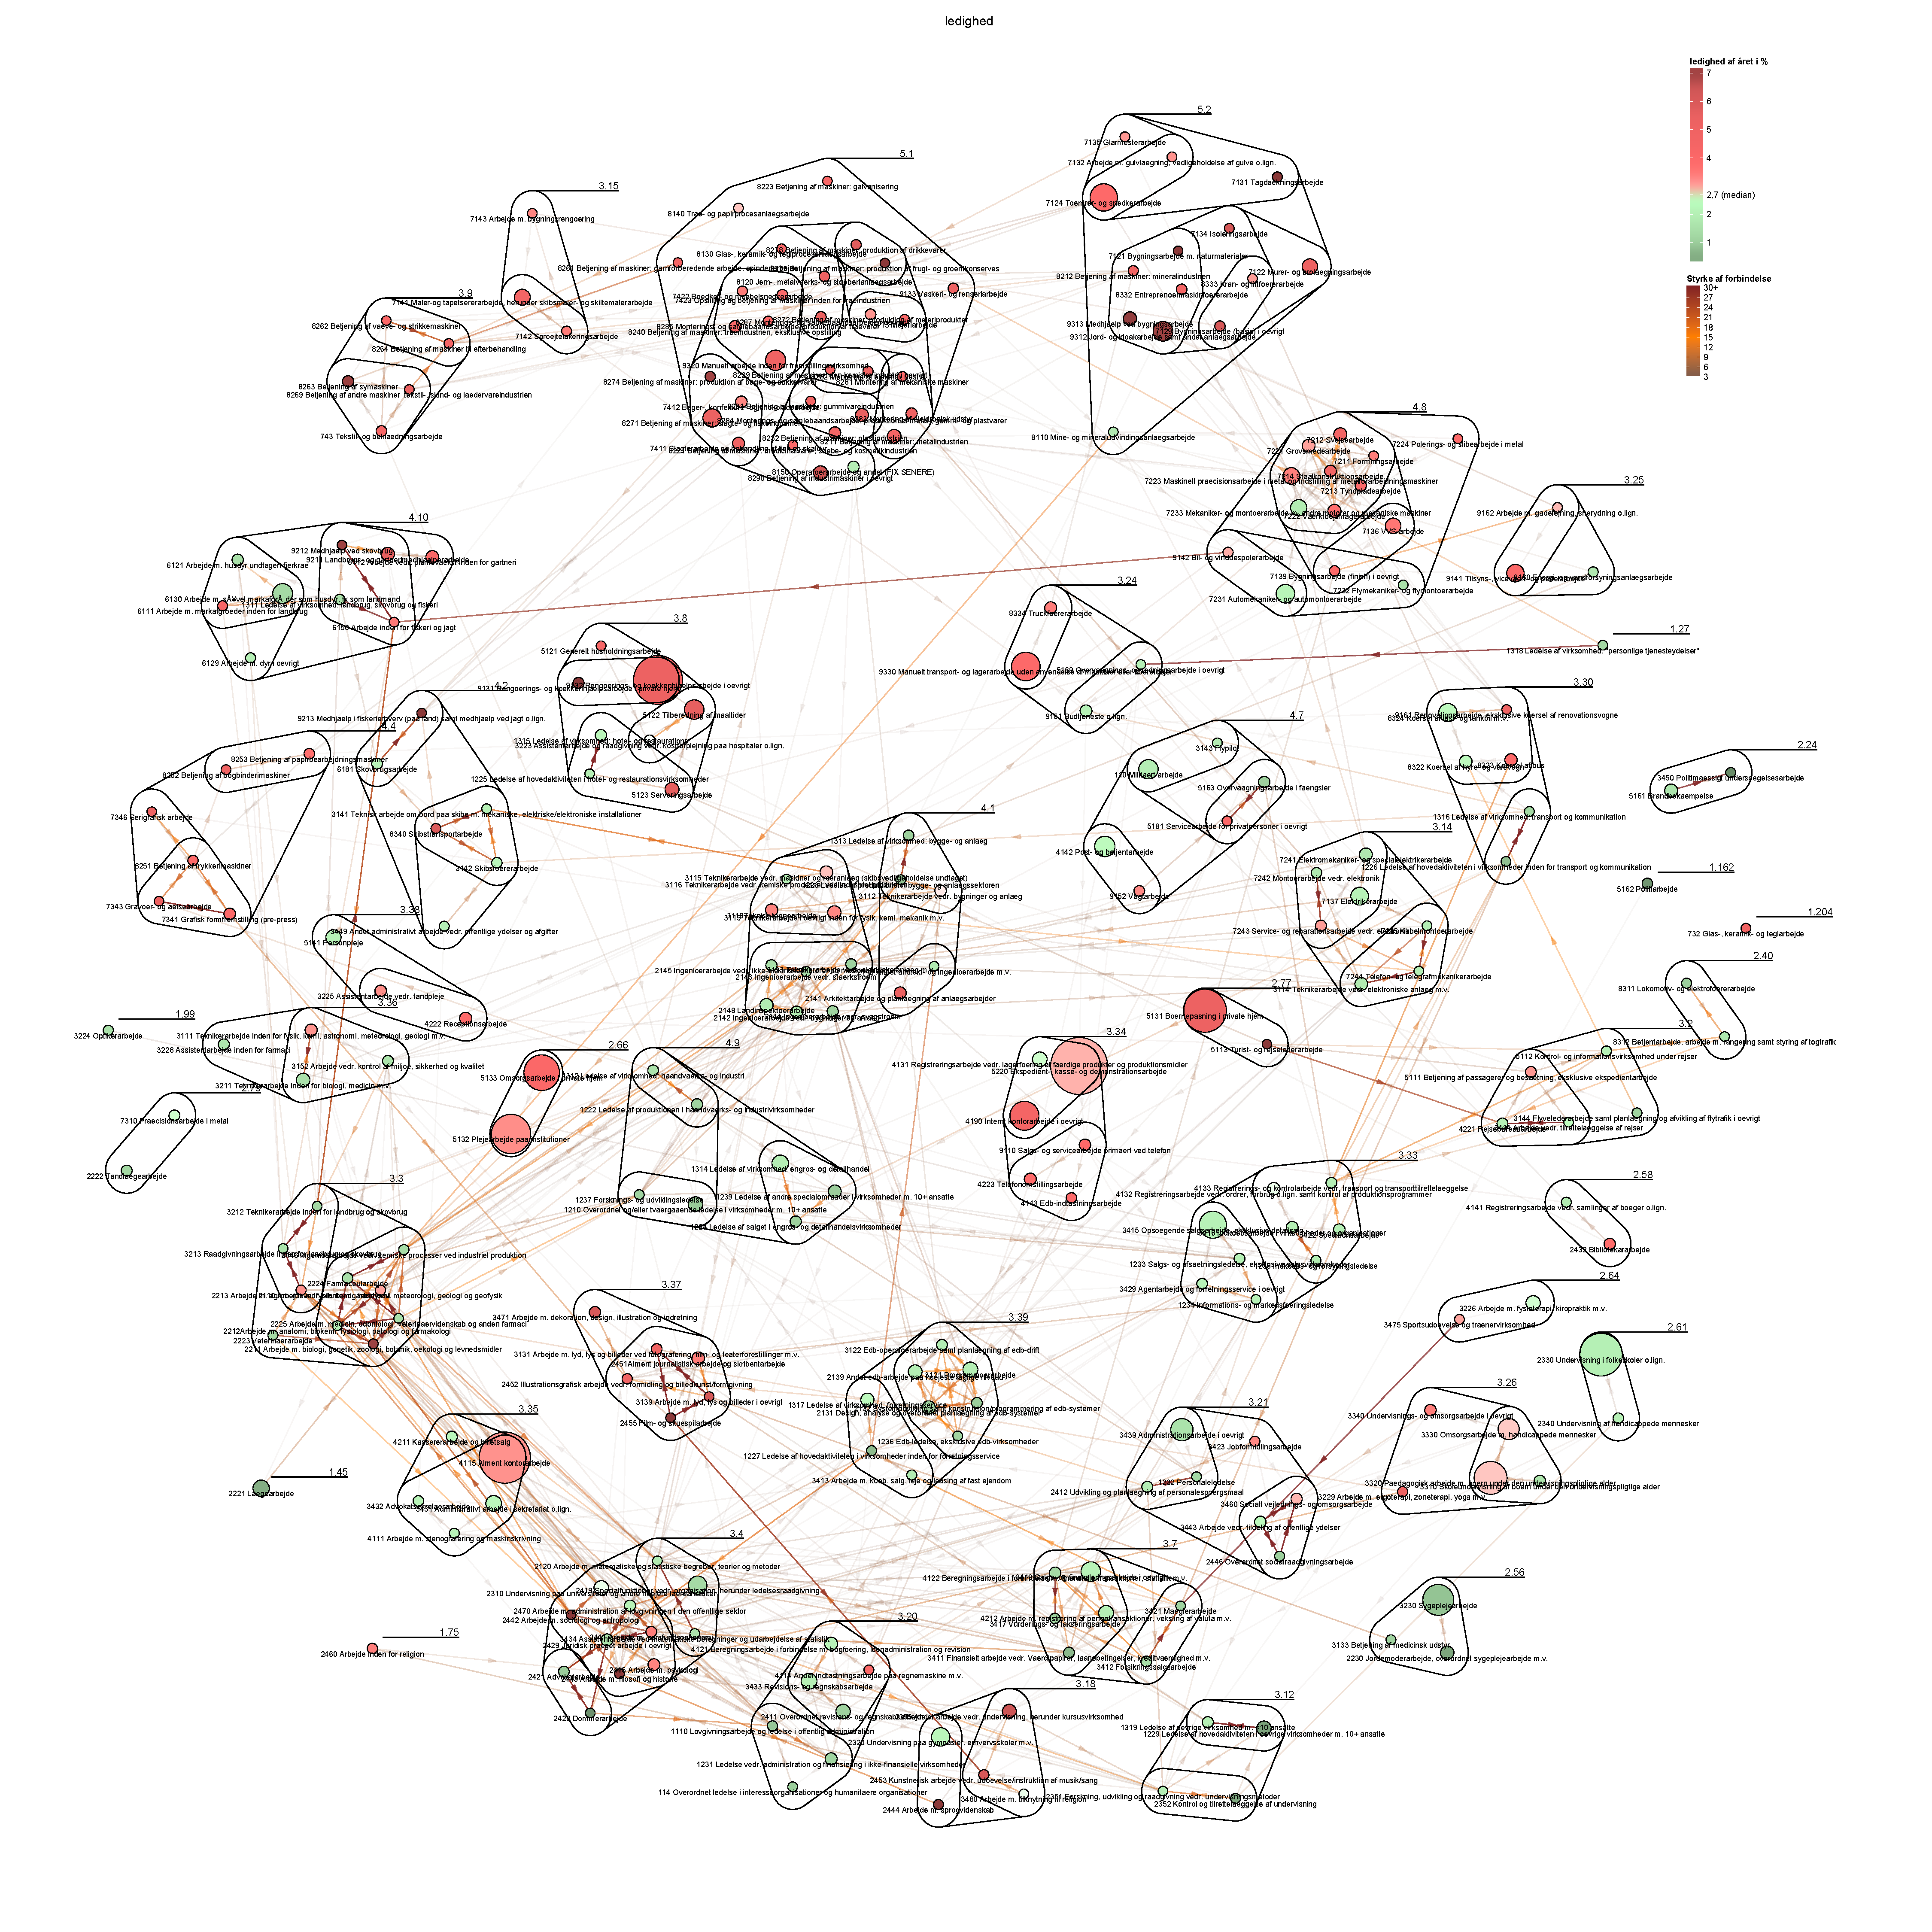
\includegraphics[width=1.0\textwidth]{fig/netvaerkskort/kort_ledighed.pdf}
\end{center}
\end{figure}
\restoregeometry
%

 
Kortet med ledighed taler knapt så tydeligt et sprog som kønskortet gør det. To af de tre segmenter, der ligger højest i ledighedsgrad, er det højkulturelle segment \emak{s3.37}, samt segment \emak{s3.18}, der indeholder kultur og undervisningsbaserede erhvervsgrupper. Først derefter kommer den del af arbejderklassen, der er beskæftiget med håndværk (\emak{s5.2}), og de, der beskæftiger sig med industriproduktion (\emak{s3.9} \& \emak{s5.1}). 

Interessant nok er det kulturelle segment og det kultur/undervisningsbaserede segment også de to segmenter, der har de absolut højeste standardafvigelser indenfor ledighed, henholdsvis 4,7 \% og 3,8 \%. 


De manuelle segmenter, derimod, varier langt mindre om gennemsnittet. En foreløbig konklusion ville derfor være, at man indenfor det kulturelle segment og det kulturelt/undervisningsbaserede segment, har langt bedre mulighed for at få et andet job indenfor samme segment, der har lavere arbejdsløshed, mens man i de manuelle segmenter ikke har samme muligheder: Der er gennemsnitttet langt mere konsistent for den generelle situation blandt alle erhvervsgrupperne i segmentet.  

Blandt segmenterne med lavest ledighed finder vi to typer jobs: Den ene er det arbejde, der udfører statens kernefunktioner; Politibetjente, læger, sygeplejersker, brandmænd og lokomotivførerer. Den anden er bestemte, højtspecialiserede typer arbejdskraft indenfor det private, men ikke \emph{hvilken-som-helst} højtspecialiseret arbejdskraft: Der er tale om ledelsessegmentet, de to finans/boligsegmenter, IT-segmentet og \emph{den ene} af de to bureaukratiske segmenter.  Hvad det skyldes er et spørgsmål om fortolkning. Der er tale om tertiære erhverv med høje uddannelseskrav, der, imodsætning til andre lignende segmenter, \emph{ikke} er rettet mod forskning, såsom det naturvidenskabelige LVU segment \emak{s3.3}. Det gælder også \emph{det andet} af de to bureaukratiske segmenter: Segment \emak{s3.4}. Dette segment indeholder højtrangerende bureaukratiske tertiære erhverv såsom advokat, ledelsesrådgivning og dommer. Det indeholder dog \emph{også} samfundsvidenskabelige jobs rettet mod akademia, og dette segment kan derfor siges at være bureakratisk-samfundsvidenskabeligt, hvilket forklarer den lavere placering i ledighedstallene. Det bureaukratisk-regnskabsrettede derimod, har ikke en sådan politisk-refleksiv karakter, men er langt mere beregnet mod varetagelse af de relativt afgrænsede, relativt klare funktioner, der findes i komplekse organisationer. 

%
\subsection{Ledighed på udvalgte delmarkeder}
%

 Jeg vil derfor zoome in på udvalgte delmarkeder og ud fra disse fortælle om de tendenser kortet viser. 

Jeg vil nu vende tilbage til det føromtalte segment \emak{s3.4}. Det har nogle interessante blah blah

Jeg vil derefter kort beskrive et segment, hvor ledigheden er nærmest identisk, for at vise noget helt andet.



%
\subsubsection{Segment 3.4: Det juridisk-samfundsfaglige segment}
%

Segment \emak{s3.4} er et segment, der består af tre niveau 2 moneca-klynger. Det ses, at det på niveau 2 er opdelt i meget klare klynger, bestemt af arbejdets genstandsfelt. I klyngen bestående af advokat- og dommerarbejde er ledigheden voldsomt lav, helt nede på 0,5 \, mens den i klyngen bestående af statistisk beregningsarbejde og specialfunktioner vedrørende ledesarbejde%
%
\footnote{ Det dækker en række forskellige jobs såsom analysekonsulent, byggesagkyndig, fuldmægtig, kommunikationskonsulent og markedsanalytiker}%
%
er på 1,5 \%, hvilket er et godt stykke under medianen på 2,6 \%. Klyngen, der trækker ledigheden væsentligt op over medianen, er “klyngen i midten”, der består af samfundsvidenskabeligt arbejde af forskellig art. Denne indeholder både “juridisk præget arbejde” såsom notar, politifuldmægtig og juridisk konsulent. Den indeholder imidlertidig også klassiske samfundsvidenskabelige discipliner såsom økonomi, sociologi, filosofi og historie%
%
\footnote{ Eller i ihvertfald \emph{samfundsrettede}.}%
%
, (højtstående) adminitrationsarbejde i den offentlige sektor, i erhvervsgruppen \emak{d2470}. 

Selvom densiteten på 67 \% vidner om en udemærket intern mobilitet, vidner denne klare forskel i ledigheden mellem på niveau 2 klyngerne internt i segmentet, at der er \emph{forskel} i de sociale processer, der styrer segmentet. Det ses afbilledet i tabel

% lav tabellen her - segment 3.4 \#todo
% indsæt tabel med 
% gennemsnitlig ledelse   
% standardafvigelse   
% antal beskæftigede    
% Andel beskæftigede   
% intern mobilitet   



Bør vi derfor, jævnfør Bojes definition af forskellen på delmarkeder og segmenter, konkludere at \emak{s3.4} ikke er et segment? Jeg vil argumentere for at et segment ikke \emph{kun} bør bestemmes ud fra en lighed i sociale processer, men også ud fra hvad jeg vil kalde \emph{sociale dynamikker}. For at forstå det, kan vi kigge nærmere på den interne mobilitet i segment \emak{s3.4}, som afbilledet i varmekortet i figur \ref{fig delanalyse2 heatmap seg3.4 ledighed}. 

% %
% \begin{wrapfigure}{r}{6cm}
%   \vspace{-20pt}
%   \begin{center}
%     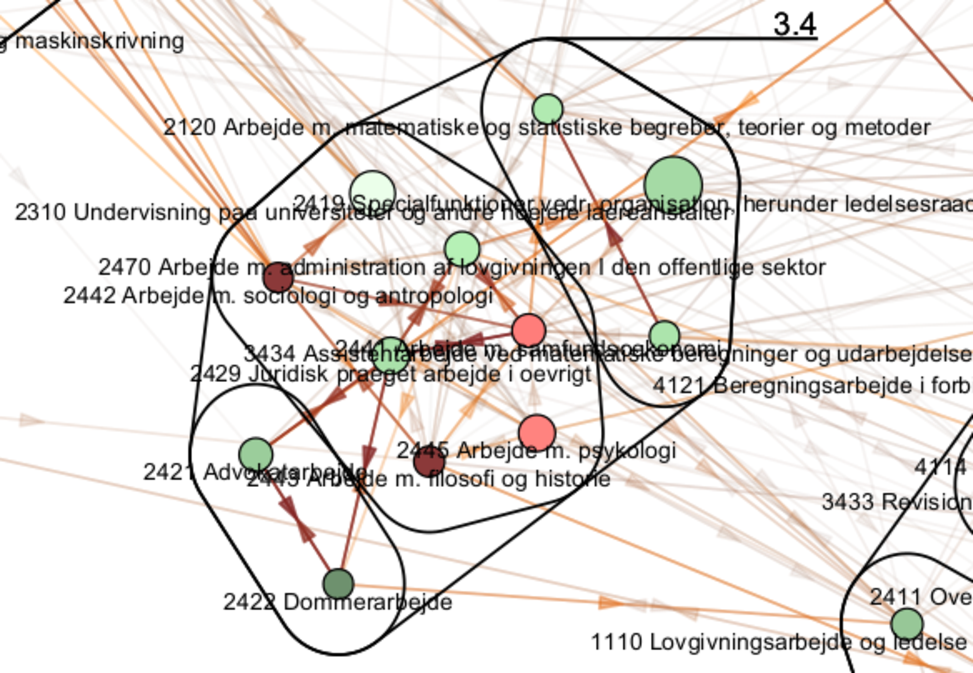
\includegraphics[width=6cm]{fig/segzoom/seg_3_4_ledighed.pdf}
%    \caption{}
%    \label{fig delanalyse2 zoom seg3.4 ledighed}
%   \end{center}
%   \vspace{-20pt}
% \end{wrapfigure}
% 
%
%
\begin{wrapfigure}{r}{10cm}
  \vspace{-20pt}
  \begin{center}
    \caption{Varmekort af segment 3.4}
      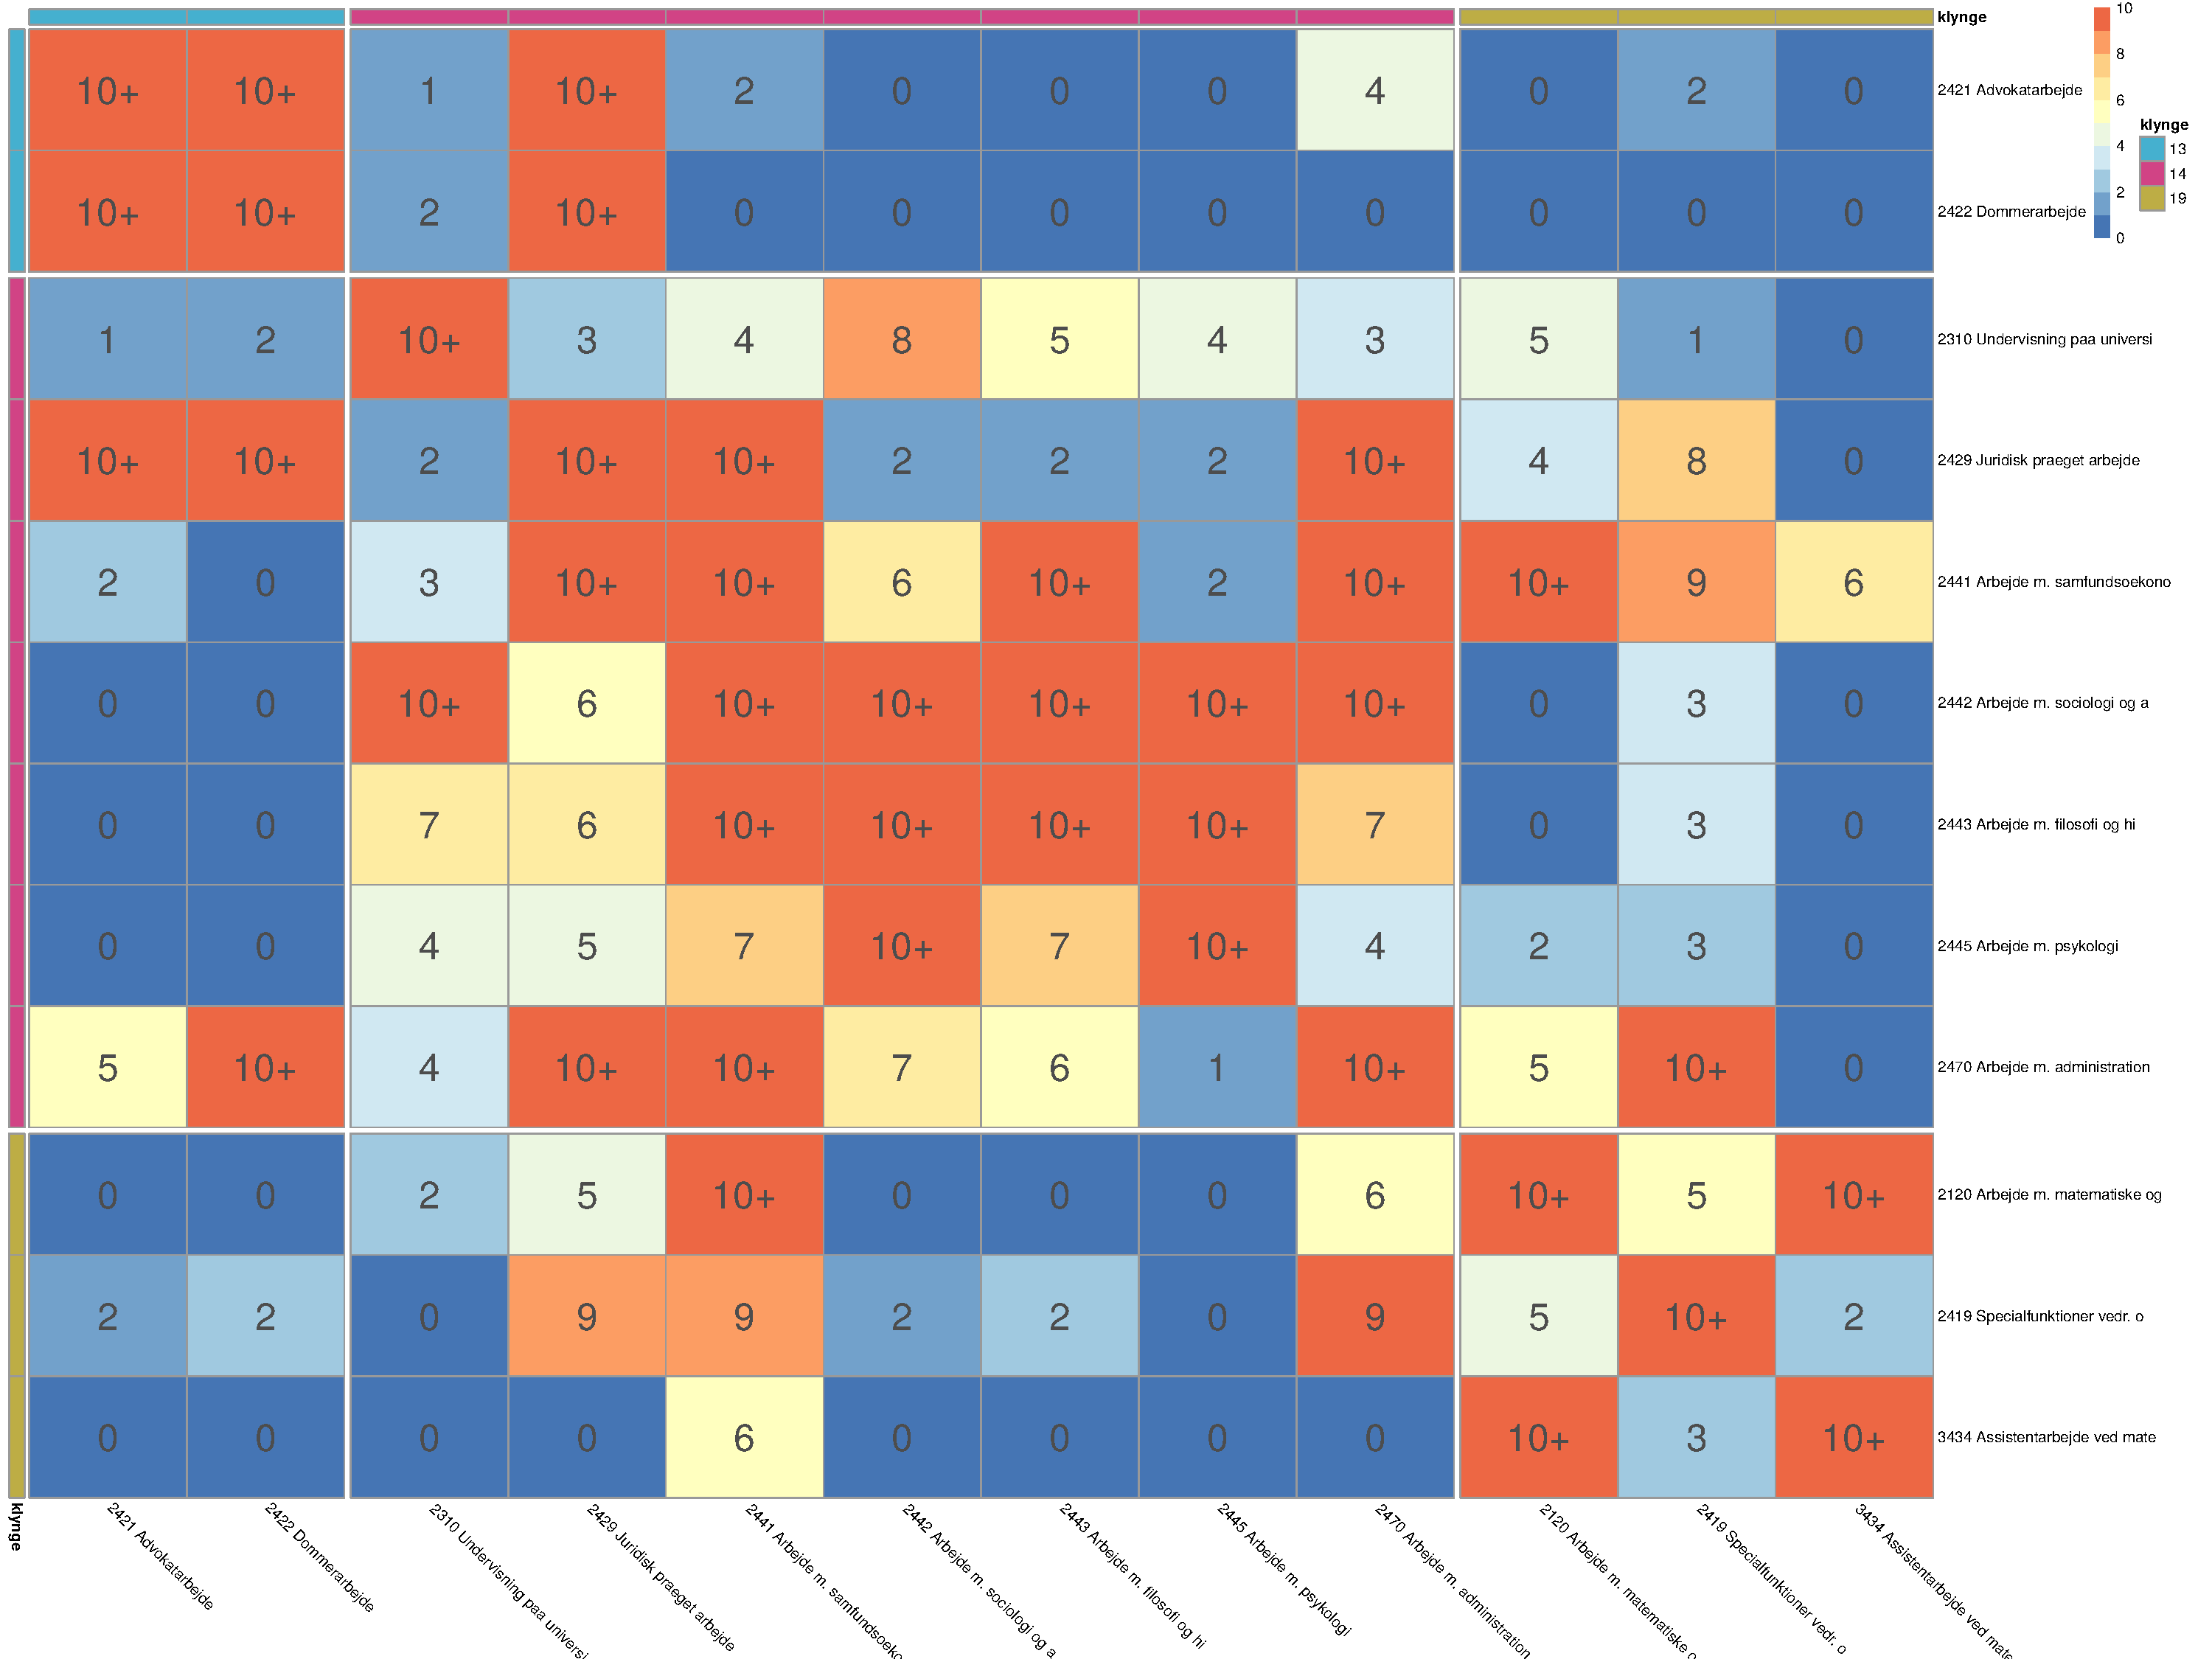
\includegraphics[width=10cm]{fig/heatmaps/seg3_4_RR_10.pdf}
    \label{fig delanalyse2 heatmap seg3.4 ledighed}
  \end{center}
  \vspace{-20pt}
\end{wrapfigure}
% %

Vi ser at der internt i klyngerne er den største interne mobilitet, hvilkket ikke er overraskende. Det interessante er at se på en klynge \emph{rækkevis}, og derefter aflæse dens mobilitet til de to andre klynger. Dette kan måske umiddelbart forekomme svært forståeligt, men en brugbar analog er en krydstabels betingede sandsynligheder: Ved at se på et udfald af en given variabel, og se dens fordeling givet en anden variabel, ser vi en sammenhæng. Det samme er tilfældet her, bortset fra at fortolkning kun er meningsfuld rækkevis, da der er en tidsdimension på spil: Vi går \emph{fra} en stilling \emph{til} en anden. 

Hvis vi ser på klyngen med dommere og advokater, kan vi se at de to erhvervsgrupper har en skyhøj intern mobilitet. Ikke så overraskende. Derefter ser vi, at denne juridiske klynge har stærke forbindelser til midterklyngen, bestående af samfundsvidenskabeligt-bureaukratisk arbejde: Det er primært \emak{d2421} , der skaber denne sammenhæng: Dommernes eneste forbindelse til de andre erhvervsgrupper, er deres undervisning på univsersiteter/højere læreranstalter samt andet juridisk præget arbejde. 

Advokaterne  derimod har stærke forbindelser til midterklyngen: dog ikke til de direkte samfundsvidenskabelige professioner som filosofi, sociologi og historie: Deres forbindelse er til de adminstrativt-juridiske professioner. \emph{Men} de samfundsvidenskabelig professioner har enormt stor mobilitet til de samme adminstrativt-juridiske erhverv som advokaterne - hvoraf nogle senere bliver dommere -, og deri sker overlappet: Forbindelsen er indrekte, men så “direkte-indirekte”, som den kan være. 

Vi ser antydningen af en genkendelig magtstruktur afspejlet, i og med at advokaterne ingen forbindelse%
%
\footnote{ “ingen forbindelse” i betydning af at den relativ risiko ikke er større, end den ville være hvis arbejdsmarkedets mobilitet var rent tilfældigt: Der \emph{er} enkelte konkrete personer, der har foretaget jobskiftet.}%
%
 har til historie, sociologi og filosofi - fag, der ikke kan siges at have meget indflydelse på hvad Bourdieu kalder magtens felt - men derimod \emph{har} har advokaterne en solid forbindelse til økonomigerningen, der må siges at have en vis indflydelse på magtens felt. Vi ser dermed konjunktuerne til en genkendelig magtstruktur, baseret på juridisk og økonomi-teoretisk fagkompetence.

Når vi taler om økonomisk-teoretisk magt, er det svært at komme udenom matematik og statistik. Dette højtspecialiseret erhverv er også tilstede i segmentet, i den sidste klynge. \emak{d2120} og \emak{d3434} har udelukkende forbindelse til de juridisk-bureaukratiske erhverv i midterklyngen, samt universitetsundervisning. Mens forbindelsen til de blødere, mere humanistisk-kulturelt orienterede samfundsfagsprofessioner som sociologi, filosofi og pyskologi glimrer ved sit fravær.

%henvis evt. til Foucualt teksten der taler om statistik som det der handler om staten - dvs magt over befolkningen. \#todo

Klyngen med statistik inkluderer også \emak{d2419}, der som beskrevet på side \pageref{d2419 forklaring} indeholder en lang række management-erhvers, hvoraf nogle i disse erhverv senere bliver både advokater og dommere. De bliver også beskæftiget med stort set alt i midterklyngen, undtagen den tungt forskningsbaserede undervisning på højere læreranstalter, samt psykologi%
%
\footnote{ hvilket overraskende - i min optik er psykologisme en stor del af managementkulturen. Men åbenbart ikke i det bureuakratisk-samfundsfaglige segment.}%
%
. 

Vi ser altså en struktur i segmentet, der har nogle bestemte mobilitetskanaler mellem erhvervsgrupperne i det. Disse kanaler er udtryk for en en bestemt social struktur, der forekommer genkendelig og rimelig, i en almen sociologisk fortolkningsramme. Det er et eksempel på hvad jeg vil kalde en \emph{social dynamik}, baseret på en hermeneutisk tilgang Monecas bud på segmentet. Til forskel fra den mere - omend på ingen måde fuldstændigt - tekniske tilgang, der ligger i at vise, at bestemte sociale fænomemer såsom løndannelse foregår ens indenfor segmentet. Jeg vil mene, at begge tilgange godtgør, at der er tale om en afgrænset del af arbejdsmarkedet, der har har nogle bestemte funktionsmåder. Jeg mener ikke at disse behøver være generiske indenfor segmentet, men der skal være tale om nogle sociale mekanismer, der godtgør en fælles platform. På denne vis har har segmenter mere tilfælles med Gruskys redefinition af klassebegrebet som mikroklasser. hvori det skal ramme en fælles livsverden, og et bestemt kulturelt funktionalistisk arbejdsfælleskab. Det vil jeg i høj grad mene er tilfældet her, og det gør det blot endnu mere interessant, at der er en ulige dynamik på spil \emph{indenfor} segmentet, der handler om, hvad man kunne kalde en nuanceforskel indenfor et bestemt genstandsfelt indenfor arbejdsmarkedet. Men en nuanceforskel, der tydeligvis ikke er ligegyldig for levevilkårene for individerne indenfor klyngerne i delmarkedet.


%
\subsubsection{Segment 3.33: blah blah }
%


Dette segment har en gennemsnitlig ledighed på 2,1 \%, hvilket er et halvt procentpoint under medianen (2,6 \%). Dette gennemsnit har samtidig en utrolig lav standardafvigelse på 0,25 \%. ledighed, forstået som social proces i Bojes forstand, rammer nærmest éns indenfor dette segment, og denne gennemsnitlige ledighed ligger endda et stykke under normalen for hele arbejdsmarkedet. 

Segmentet består af to klynger. Det ene indeholder de erhverv, der håndterer den \emph{hovedsageligt} logistiske transport og allokering af varer%
%
\footnote{ I modsætning til den helt konkrete fysiske transport af varer fra A til B, der varetages af segment 3.24 og 3.30. Det er ufaglært arbejde i Discos hovedgruppe 8 og 9.}%
%
 i samfundet: Jobs som distributionschef, tolder, importagent og speditør er de mere administrativt prægede, men det inkluderer også jobs som godsekspedient, luftfartsassistent og garagemester, der mere direkte håndterer varernes fysiske bevægelse fra A til B.


% 
\begin{wrapfigure}{r}{6cm}
  \vspace{-20pt}
  \begin{center}
    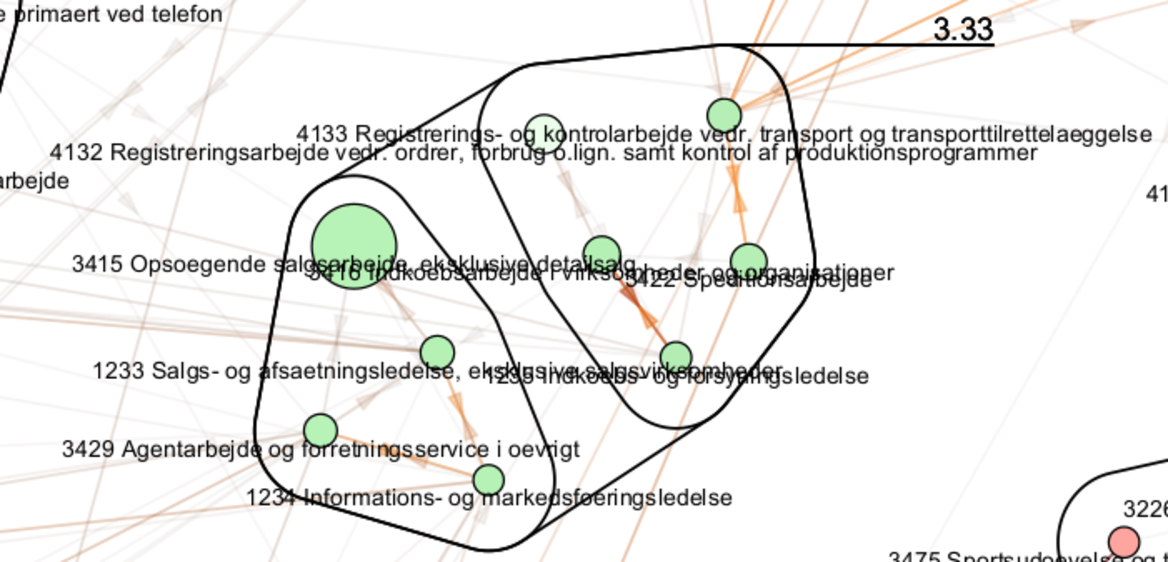
\includegraphics[width=6cm]{fig/segzoom/seg_3_33_ledighed.pdf}
   \caption{}
   \label{fig delanalyse2 zoom seg3.33 ledighed}
  \end{center}
  \vspace{-20pt}
\end{wrapfigure}
%

Den anden klynge består af erhvervsgrupper der sørger for \emph{allokeringen} af varerne på markedet: Salgsfasen, inklusiv reklamearbejdet. Her finder vi også to erhvervsgrupper fra Discos ledelsesklynge, \emak{d1234}. Det betyder at både jobs som marketingschef og reklamechef findes i klyngen, sammen med jobs som salgsagent, sælger, reklameassistent og eksportagent. Vi kan ud 

Dette segment har altså en klar funktion i samfundet, der dækker to centrale aspekter af varenes cyklus. Dette fordrer - eller kovarierer ihvertfald med -  en meget ensartet ledighedsrate%
%
\footnote{ Det er i øvrigt også sandt over tid, i perioden 1996-2009.}%
%


%
\subsection{Her burde nok stå noget klogt til at konkludere }
%

Lorem ipsum dolor sit amet, consectetur adipisicing elit, sed do eiusmod
tempor incididunt ut labore et dolore magna aliqua. Ut enim ad minim veniam,
quis nostrud exercitation ullamco laboris nisi ut aliquip ex ea commodo
consequat. Duis aute irure dolor in reprehenderit in voluptate velit esse
cillum dolore eu fugiat nulla pariatur. Excepteur sint occaecat cupidatat non
proident, sunt in culpa qui officia deserunt mollit anim id est laborum.



%%%%%%%%%%%%%%%%%%%%%%%%%%%%%%%%%%%%%%%%%%%%%%
\section{fagforeninger \label{sec_delanalyse2 fagforeninger}}
%%%%%%%%%%%%%%%%%%%%%%%%%%%%%%%%%%%%%%%%%%%%%%

fagforeninger løndannelse vigtigt  segmenter Lorem ipsum dolor sit amet, consectetur adipisicing elit, sed do eiusmod
tempor incididunt ut labore et dolore magna aliqua. Ut enim ad minim veniam,
quis nostrud exercitation ullamco laboris nisi ut aliquip ex ea commodo
consequat. Duis aute irure dolor in reprehenderit in voluptate velit esse
cillum dolore eu fugiat nulla pariatur. Excepteur sint occaecat cupidatat non
proident, sunt in culpa qui officia deserunt mollit anim id est laborum.


%
\subsection{fagforeninger på arbejdsmarkedet }
%

I figur \ref{fig_delanalyse1_kort_ledighed} på side \pageref{fig_delanalyse1_kort_ledighed} ser vi netværkskortet farvelagt efter organiseringsgraden i LO-fagforeninger. Af grunde fremlagt i bilag \ref{app_fagforening} er dette tal upålideligt for tjenestemænd: Derfor har en række erhvervsgrupper bestående af tjenestemænd en svagt XXX farve på kortet.  


% Det er i det hele taget et billede, der gør sig gældende: De segmenter, der har en standardafvigelse i organiseringsgraden på under 10 \% - det vil sige et lille stykke under medianen - er ikke nødvendigvis bedre uddannede, men mange af dem har arbejde, der typisk fordrer en ansættelse indenfor staten. Undtagelserne er det lille segment \emaks{3.15}, der består af malere og autolakerer,  → nej, det gør sig faktisk ikke gældende, fordi de ikke er særligt *højt* organiserede.



%
\newgeometry{left=-0.01cm,bottom=0.1cm}
\begin{figure}[H]
\begin{center}
  \caption{organiseringsgrad i delmarkederne}
  \label{fig_delanalyse2_kort_roed}
  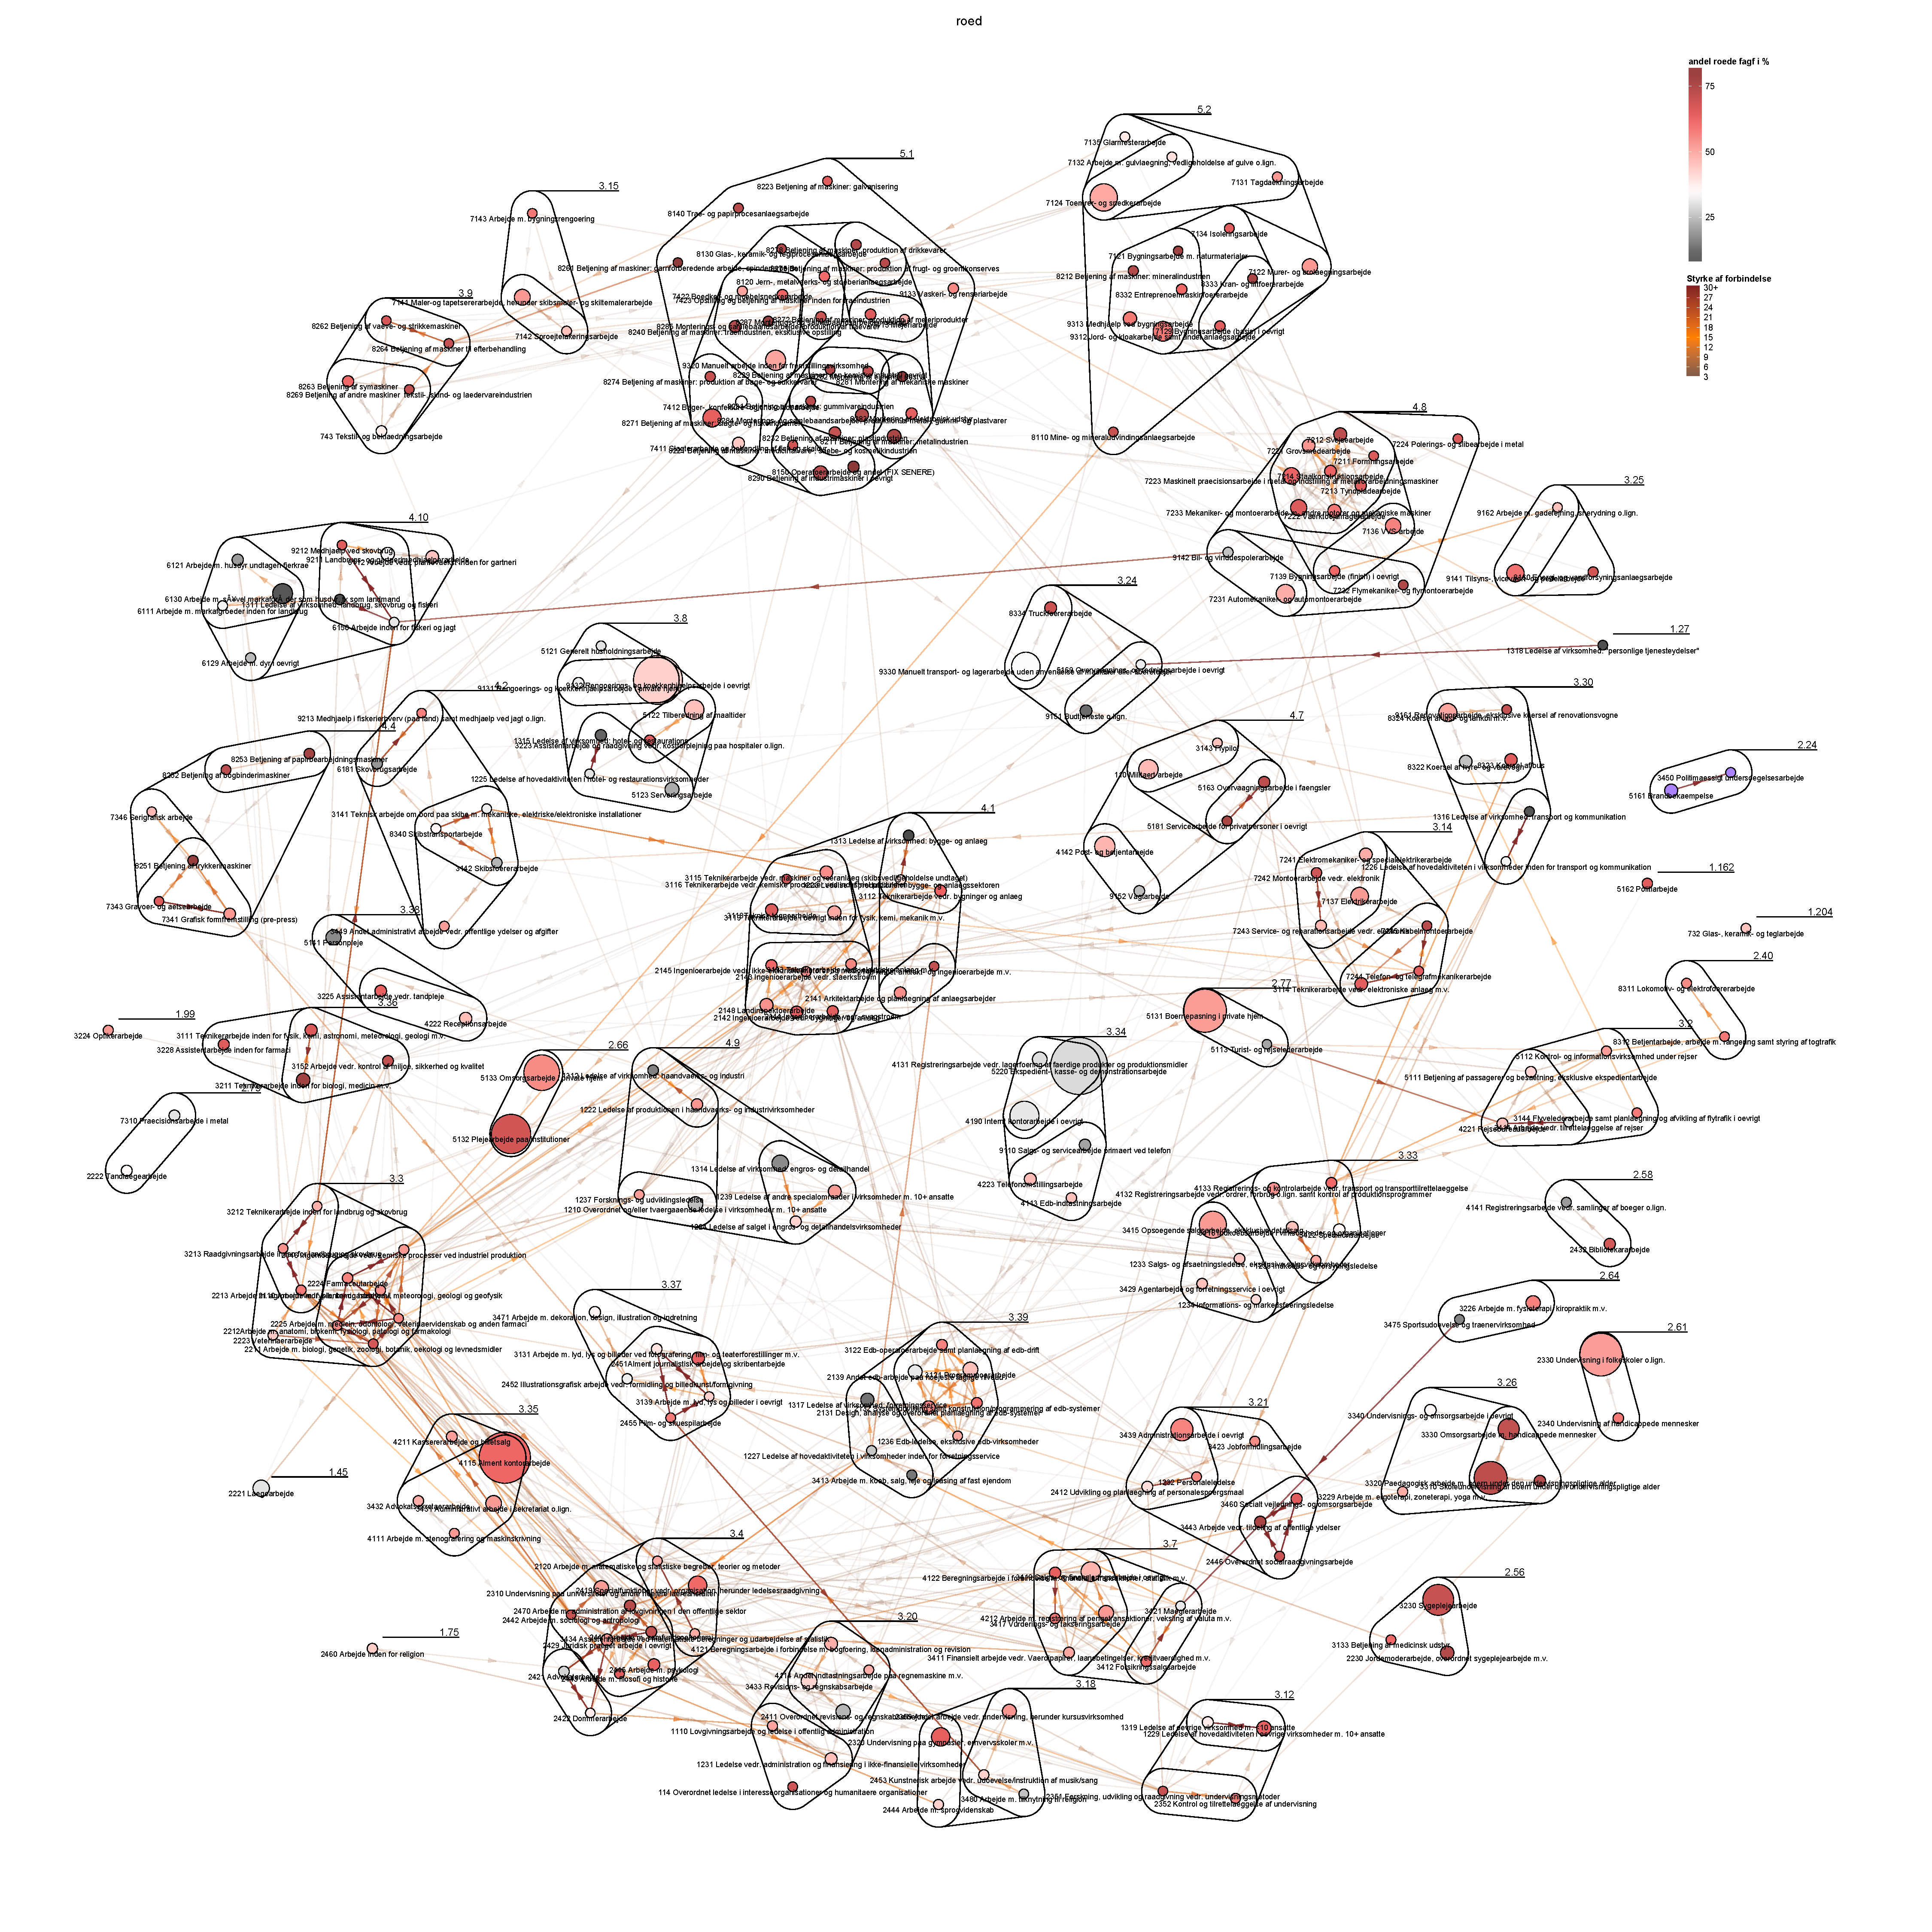
\includegraphics[width=1.0\textwidth]{fig/netvaerkskort/kort_roed.pdf}
\end{center}
\end{figure}
\restoregeometry
%

Der kan peges på nogle overordnede tendenser. Den første er at de tre segmenter med højest organiseringsgrad bemærkelsesværdigt lader til at have tre vidt forskellige sociale modaliteter. De bedst organiserede  erhvervsgrupper befinder sig i segment \emak{s3.36}. Det er arbejde af naturvidenskabelig karakter, der ikke kræver en universitetsuddannelse, og som primært beskæftiger sig med (assisterende) laboratoriearbejde og kvalitetskontrol af (føde)varer og (arbejds)miljø. Disse er tilsyneladende særdeles godt organiseret, hvilket kan skyldes deres organisering i som embedsmænd (???? \#todo få Martin til at hjælpe dig med det her). efter det kommer sygeplejersker, jordemødre, radiograf og andre beskæftiget indenfor sundhedssektoren, altså offentligt ansatte indenfor sundhedssektoren på et mellemlangt uddannelsessniveau. 

Derefter kommer den del af arbejderklassen, der arbejder manuelt, og som ikke har særlig meget uddannelse. Overraskende nok er deres organiseringsgrad en del bedre end håndværkerne i klynge \emak{s4.8} og \emak{s5.2}. Dog er standardafvigelsen for de manuelle arbejder-segmenter på omtrent 13 \%, hvilket svarer til den gennemsnitslige standardafvigelse for organiseringsgraden indenfor alle segmenterne, mens den for de føromtalte sygeplejerske- og varekontrol segmenter ligger på 7 \%. I disse manuelle dele af arbejderklassen er organiseringsgraden derved langt mere variende indenfor erhvervsgrupperne, end for de føromtalte. 

Der er ikke et klart mønster, i hvilke segmenter der har en lav standardafvigelse i organiseringen, og hvilke, der har en høj. Segment \emak{s2.79} med tandlæger og præcisionsarbejder i metal, har en stabilt \emph{lav} organiseringsgrad, mens “DSB”-segmentet, \emak{s2.40}, bestående af lokomotivfører og anden jernebanerelateret arbejde, har en stabilt \emph{høj} organiseringsgrad. 

Den anden tendens, der kan spores, er at landbrugsrelaterede erhverv har en lav faglig organisering.

%%%%%%%%%%%%%%%%%%%%%%%%%%%%%%%%%%%%%%%%%%%%%%
\section{Udvalgte delmarkeders faglige organisering \label{sec_delanalyse2 udvalgtedelmarkeder fagforening}}
%%%%%%%%%%%%%%%%%%%%%%%%%%%%%%%%%%%%%%%%%%%%%%

%
\subsubsection{Segment 5.1: Fabriksarbejderne}
%




Det første segment vi ser på er den føromtalte \emak{s5.1}. Denne er interessant, fordi den udgør hele 6,4 \% af arbejdsstyrken, og er et kernesegment i den manuelle del af arbejderklassen. Der er en del forskel på hvordan klyngerne internt i segmentet er fagligt organiserede, hvilket bliver klart ud fra følgende:

%du kunne evt. lave en mini-moneca og vise hvorden de ser ud i klyngenre. \#todo.

%
\begin{wrapfigure}{r}{6cm}
  \vspace{-20pt}
  \begin{center}
    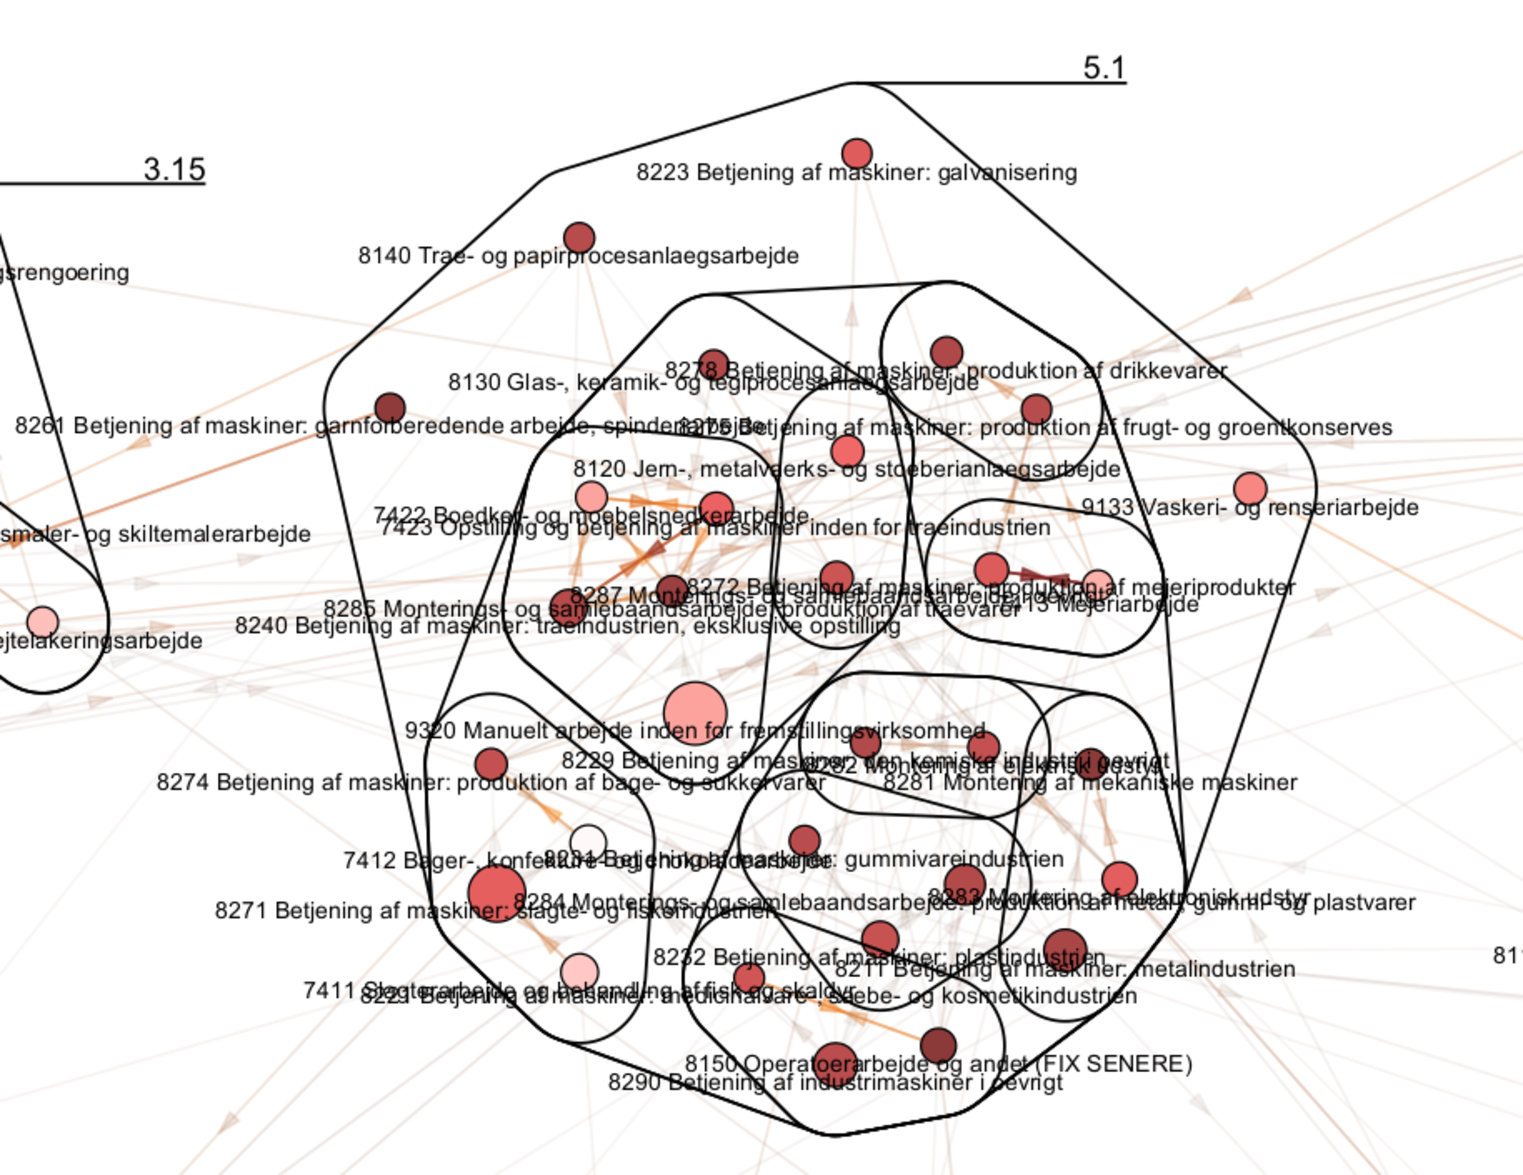
\includegraphics[width=6cm]{fig/segzoom/seg_5_1_roede.pdf}
   \caption{}
   \label{fig_delanalyse2_zoom_3_4 koen}
  \end{center}
  \vspace{-20pt}
\end{wrapfigure}
%

Klynge 3.17 udgør hovedbestandelen i segmentet. Den sociale proces, vi kigger på - faglig organisering - er rimelig ensartet og særdeles høj, med et gennemsnit på 74 \%. Den er således en faglig bastion både internt i segmentet, men har samtidig en størrelse, der gør at den også er det i samfundet som sådan. Klynge 3.10 og 3.16 er også godt med, omend der i hver af disse to klynger er henholdsvis én og to erhvervsgrupper, der har væsentlig lavere faglig organisering end resten. i Klynge 3.10 er det \emak{d7413}, der stikker ud fra resten af klyngen, ved at være et landbrugsbaseret erhverv fremfor et industrierhverv. Ved at se på mobiliteten mellem erhvervsgrupperne i klyngen såvel som i segmentet som helhed, er mejerist et erhverv, folk næsten udelukkende kommer \emph{fra}. Vi ved at de landbrugsbaserede erhverv har en lavere faglig organiseringsgrad. Denne formodning styrkes ved at se på mobiliten for mejerister ikke bare i segment 5.1, men til alle andre beskæftigelser: At gå fra at være mejerist til noget andet er et \emph{make it or break it} punkt, statistisk set: en lille gruppe går til et ledelses/arbejdsgiver-erhverv indenfor \emak{d1222}. De resterende går til forskellige former for manuelt arbejde, primært indenfor segment 5.1. Mejerist ser derfor ud til at være et overgangserhverv fra en landbrugsbaseret arbejdskultur til en industriel arbejdskultur. Derfor er den inkluderet i segment 5.1, og derfor er dens faglige organisering så meget lavere: Det er først i mødet med indutrikulturen i resten af klyngen og segmentet, at organisering finder sted%
%
\footnote{ Om det er de tidligere mejerister der står for den del af de uorganiserede i de erhverv, de bevæger sig hen til, er et spadestik for dybt for denne meso-fokuserede analyse af arbejdsmarkedet. Men tanken er interessant: Er landbrugskulturen så dybt forankret i individerne, at de vedbliver med at være uorganiserede i resten af deres livsbane, eller forandrer industrikulturen dem?}%
%

I klynge 3.16 er det sværere at finde en lignende historie: Jeg må bare konstarere, at i en analyse på dette plan, er det bare sådan, det er: Det ville kræve et andet detaljeniveau at finde årsagerne.

Det sidste der skal bemærkes om dette segment er, at at den klynge, der for alvor trækker gennemsnittet ned, er to af erhvervsgrupperne i klynge 2.42. I modsætning til deres klyngefæller ikke beskæftiget med betjening af maskiner. Om det er det, der gør forskellen, er svært at udtale sig om, men det er en nærliggende tanke. Det er muligvis fordi, der findes flere selvstændige i denne gruppe, og det ligger tæt på en småborgerlig kultur (forsøg at definer den med Bourdieu, måske et afsnit fra Distinktionen, måske det der der er med i DDS pensum \#todo)

%
\subsubsection{Segment 3.35 \& 3.34: De organiserede og de uorganiserede servicearbejdere }
%

Lorem ipsum dolor sit amet, consectetur adipisicing elit, sed do eiusmod
tempor incididunt ut labore et dolore magna aliqua. Ut enim ad minim veniam,
quis nostrud exercitation ullamco laboris nisi ut aliquip ex ea commodo
consequat. Duis aute irure dolor in reprehenderit in voluptate velit esse
cillum dolore eu fugiat nulla pariatur. Excepteur sint occaecat cupidatat non
proident, sunt in culpa qui officia deserunt mollit anim id est laborum.

Skriv kun måske det her afsnit. Måske ikke så vigtigt. 





%                               ¤                             #



\iffalse


########## ideer til analyser / pointer ###################

Konkludere på kravet med social proces. Tydeligvis stor forskel. Grusky har ret, tingene er professionsbaseret. Der findes ikke en samlet arbejderklasse. %fractured among occupational lines, som Grusky siger. 


røde halvmåne og grønne formation - men de er jo ikke helt udtryk for moneca kortet, udover en algoritme der laver det forskelligt hver gang. Hmm. 

hvor mange kvinder indenfor ledelse fx 


lav skal der definerer dem der er røvrendt på alle parametre, dvs både indenfor ledighed og timeløn ligger de under medianen. Eller, måske er det ikke så underligt at man ligger under medianen når man har det ene og det andet. Måske skal analysen mere være: Hvem er særligt privilegierede, i og med de har højere ledighed og stadig høj timeløn? Kan man det? Det handler også om det tekniske i at de to mål muligvis er afhængige af de samme beregniner, problematisk. 


De personer som arbejder og skifte job inden for delmarked \emak{s3.4} arbejder som advokater, dommere, sociologer, antropologer, statistikere, undervisere på universitetere, historikere, filosoffer, psykologer. De får en løn som i gennemsnit spænder fra XXX kr/time for de laveste (hvem er det) til XXX kr/time (hver er det). Udover en høj timeløn har de det til fælles at det typisk kræver en lang videregående uddannelser for at besidde disse job. Nogle jobs såsom advokat- og dommerarbejde har kræver udover en lang videregående uddannelser og en særlig efteruddannelse.

De personer som arbejder og skifte job inden for delmarked \emak{s5.1} arbejder som slagtere, bagere, mejerister, arbejde med betjening af maskiner, monteringsarbejde, samlebåndsarbejde og manuelt arbejde. De får en løn som i gennemsnit spænder fra XXX kr/time for de laveste (hvem er det) til XXX kr/time (hver er det) med en enkelt afstikker på XXX kr/time. Udover en lavere timeløn har de det til fælles at det typisk kræver en erhvervsuddannelse eller et kortere kursus at besidde disse job.

Den første umiddelbare umiddelbare forklaring på lønsforskellen mellem de to segmenter er uddannelse. For at arbejde inden for de to delmarkeder kræver det en uddannelse. Forskellen er så længden på uddannelsen. Det er anerkendt, at der er en sammenhæng mellem uddannelse er løn. Human kapital er en økonomisk teori udviklet af Gary Becker, der beskriver, at arbejdstagere kan tage en uddannelse som en investering mod forventning om økonomisk kompensation ved at vedkommendes produktivitet øges (fx Cahub og Zylberberg 2004, s. 69). Da de akademiske uddannelser tager længere tid end erhvervsuddannelser og kortere kursus, giver det også en højere økonomisk kompensation. 





Attributterne er ikke anvendt som inklusionskriterier og kan derfor bruges til at
vurdere, hvorvidt der er overensstemmelse mellem privilegerede positioner i netvær-
ket og symbolske eller økonomiske privilegier, der er eksterne for netværket. Dette giver
os mulighed for at vurdere om vores specifikation af netværket stemmer overens med
magtsymboler, hvilket kan benyttes til at vurdere validitet ( 1983, s. 29).


validitet i et klasseskema: ekstern og intern validitet (Oesch s. 94)

indkomst som udtryk for magt på arbejdsmarkedet og social status. Dermed "den afgørende faktor" for menneskers livschancer. s. 95

Boje peger på faren ved at fokusere på outcomet af sociale processer såsom lønforskelle, arbejdsløshed, hyppige jobskifte m.m.. Det er en reel fare ved mit empiriske arbejde. s. 28, men meget god hvis man vil sikre sig at alt er, som det skal være. 

Grundet den danske struktur og fokus på organisering må det forventes, at mobilitets- og lønbarrierer primært findes indenfor fag, og ikke indenfor industrier/erhvervsgrene, hvilket findes i USAs langt mindre organiserede og mere monopolitiske virksomhedskultur. 

"i perioder med økonomisk tilbagegang og hvor der på arbejsmarkedet er overudbud af lønarbejdere synes barriererne mellem segmenterne at blive skærpet." (...) og nye segmenter og delmarkeder opstår på den baggrund. s. 72
→ perioden 1996-2009 er en periode med vækst, dvs: Det her en god periode. Find tal for økonomisk vækst for perioden


brug relative forskel mellem lønninger, ikke bare den absolutte, som må siges at være den vigtigste for personerne selv. Brug medianen for den "nederste klasse" som udtryk for lønniveauet. Kan du overføre det til dit eget? lønniveauet for den lavest tjenende klynge?

Oesch afviser at "future prospects" skulle have stor betydning, da han mener at påvise en stærk sammenhæng mellem nuværende lønninger og fremtid indkomst. I danmark, viser Esping-Andersen, fungerer low-income jobs sådan. Men vi kan jo se, hvor folk bevæger sig hen. Og det ser ikke ud til at være en stærk sammenhæng mellem service-jobs og future prospects. Undersøg servicejobs og ande


find ud af hvor mange skift der er per år. Dejligt konkret tal. henvis til boje 1988 s. 123


Løndannelsen s. 79-80
	i det sekundære arbejdsmarked synes der ikke at være en sammenhæng mellem løn og uddannelse - det er ikke det, der er det centrale. Hvorimod på det primære arbejdsmarked synes det netop at være betydningsfuldt, her er uddannelsesmæssige ressource nøje afstemt med løn. 
	tre forhold spiller ind:
	- institutionel regulering kontra markedsregulering: I DK er stort set al løndannelse reguleret gennem institutionelle aftaler 
	→ har nok ændret sig noget siden, men i det store og hele nok stadig rigtigt
	- Lønnen knyttet til job kontra til præstation.
	- lønnen tilnyttet stillingsmæssigt avancement/ikkeavancement. primære forskel på sekundær/primær løn. det sekundære jobmarked har samme lønninger livet igennem. 





















% %%%%%%%%%%%%%%%%%%%%%%%%%%%%%%%%%%%%%%%%%%%%%%
% \section{kønsforskelle i sociale processer \label{sec_delanalyse2_køn}}
% %%%%%%%%%%%%%%%%%%%%%%%%%%%%%%%%%%%%%%%%%%%%%%

% En grundlæggende differentieringsform i snart sagt alle samfund er



%  kønsopdelingen, der kommer til udtryk i en kønsbestemt arbejdsdeling i langt de fleste samfund. Som David Oesch bemærker, er det påfaldende, hvor få kvantitative undersøgelser af arbejdsmarkedsrelationer, der inddrager køn i analyserne  














\fi


